\section{The SSU ribosomal RNA secondary structure models used by \textsc{ssu-align}}

The profile probabilistic models of SSU rRNA in \textsc{ssu-align} are
derived from the alignments generated by Robin Gutell and colleagues
at the University of Texas Austin \cite{Cannone02}. There are 5 CM
files, each was constructed from a separate alignment from the
Comparative RNA Website as explained below.

\subsection{SSU rRNA data available from the Comparative RNA Website}

The Comparative RNA Website (CRW) is an extremely valuable for
sequence and structure data on many structural RNAs including small
subunit ribosomal RNA, large subunit ribosomal RNA, 5S and 5.8S
ribsomal RNA, group I and group II self-splicing introns. For the
purpose of building SSU rRNA CMs, the most relevant information
available from CRW is multiple alignments and individual secondary
structures that were determined using comparative analysis for a
subset of the sequences available in the alignments. 

TO DO.

\begin{comment}
\textsc{infernal} builds a CM from a consensus structure annotated
multiple sequence alignment. So, to use the CRW data I had to develop
a pipeline that mapped the individual structures onto the alignments
and then derived a consensus structure from the individual structures.

I decided to first extract only the sequences that had individual
structure information from the larger alignments, 

Because the unique feature of CM SSU alignment relative to other existing
methods is it's ability to take secondary structure into account
during alignment the most important information from CRW 

\textsc{infernal} builds sequence and structure profiles of an RNA
sequence family from a multiple alignment of 
\end{comment}

\subsection{Deriving consensus structure annotated \emph{seed} alignments from CRW data}

TO DO.

\subsection{Building CMs from seed alignments}

\textsc{infernal}'s \prog{cmbuild} program builds CM files from
consensus structure annotated alignments. \textsc{ssu-align} includes
the five default training alignments (named \prog{<family>.stk}, where
\prog{<family>} is either archaea, bacteria, chlorplast, eukarya or
metamito) as well as the five CMs resulting from them (named
\prog{<family>.cm}). (The metamito model is a metazoan mitochondria
model). The models were built using \prog{cmbuild} as
follows: 

\user{cmbuild --enone --gapthresh 0.8 archaea.cm archaea.stk}

\begin{comment}
The default behavior and parameters of \prog{cmbuild} have been
optimized to build CMs that are sensitive to remote homology detection
in homology search applications (the main application of CMs)
\cite{Nawrocki07}. But when building CMs for accurate SSU rRNA
alignment a few parameters can be tweaked to get better
performance. 
\end{comment}

MORE ON WHY THESE OPTIONS WERE USED.

\subsection{Seed alignment and model statistics} 

% stats from esl-alistat and cmbuild-1.0 on ssu5-0p1.stk
\begin{center}
\begin{tabular}{lrrrrrr}
        &           &           &           &           & average   & average  \\
model   & number of & consensus & alignment & number of & sequence  & pairwise \\
name    & sequences & length    & length    & basepairs & length    & identity \\ \hline
        &           &           &           &                       &          \\
archaea & 23        & 1508      & 1563      & 471       & 1485      & 81\%     \\
bacteria& 93        & 1582      & 1689      & 480       & 1527      & 80\%     \\
chloroplast& 18     & 1514      & 1693      & 449       & 1492      & 85\%     \\
eukarya  & 89       & 1881      & 2652      & 448       & 1800      & 79\%     \\ 
metamito & 55       &  996      & 1127      & 256       & 957       & 76\%     \\
\end{tabular}
\end{center}

\subsection{Secondary structure diagrams of seed alignments}

TO INCLUDE: HEATMAPS of the 5 models.

\begin{center}

\newpage
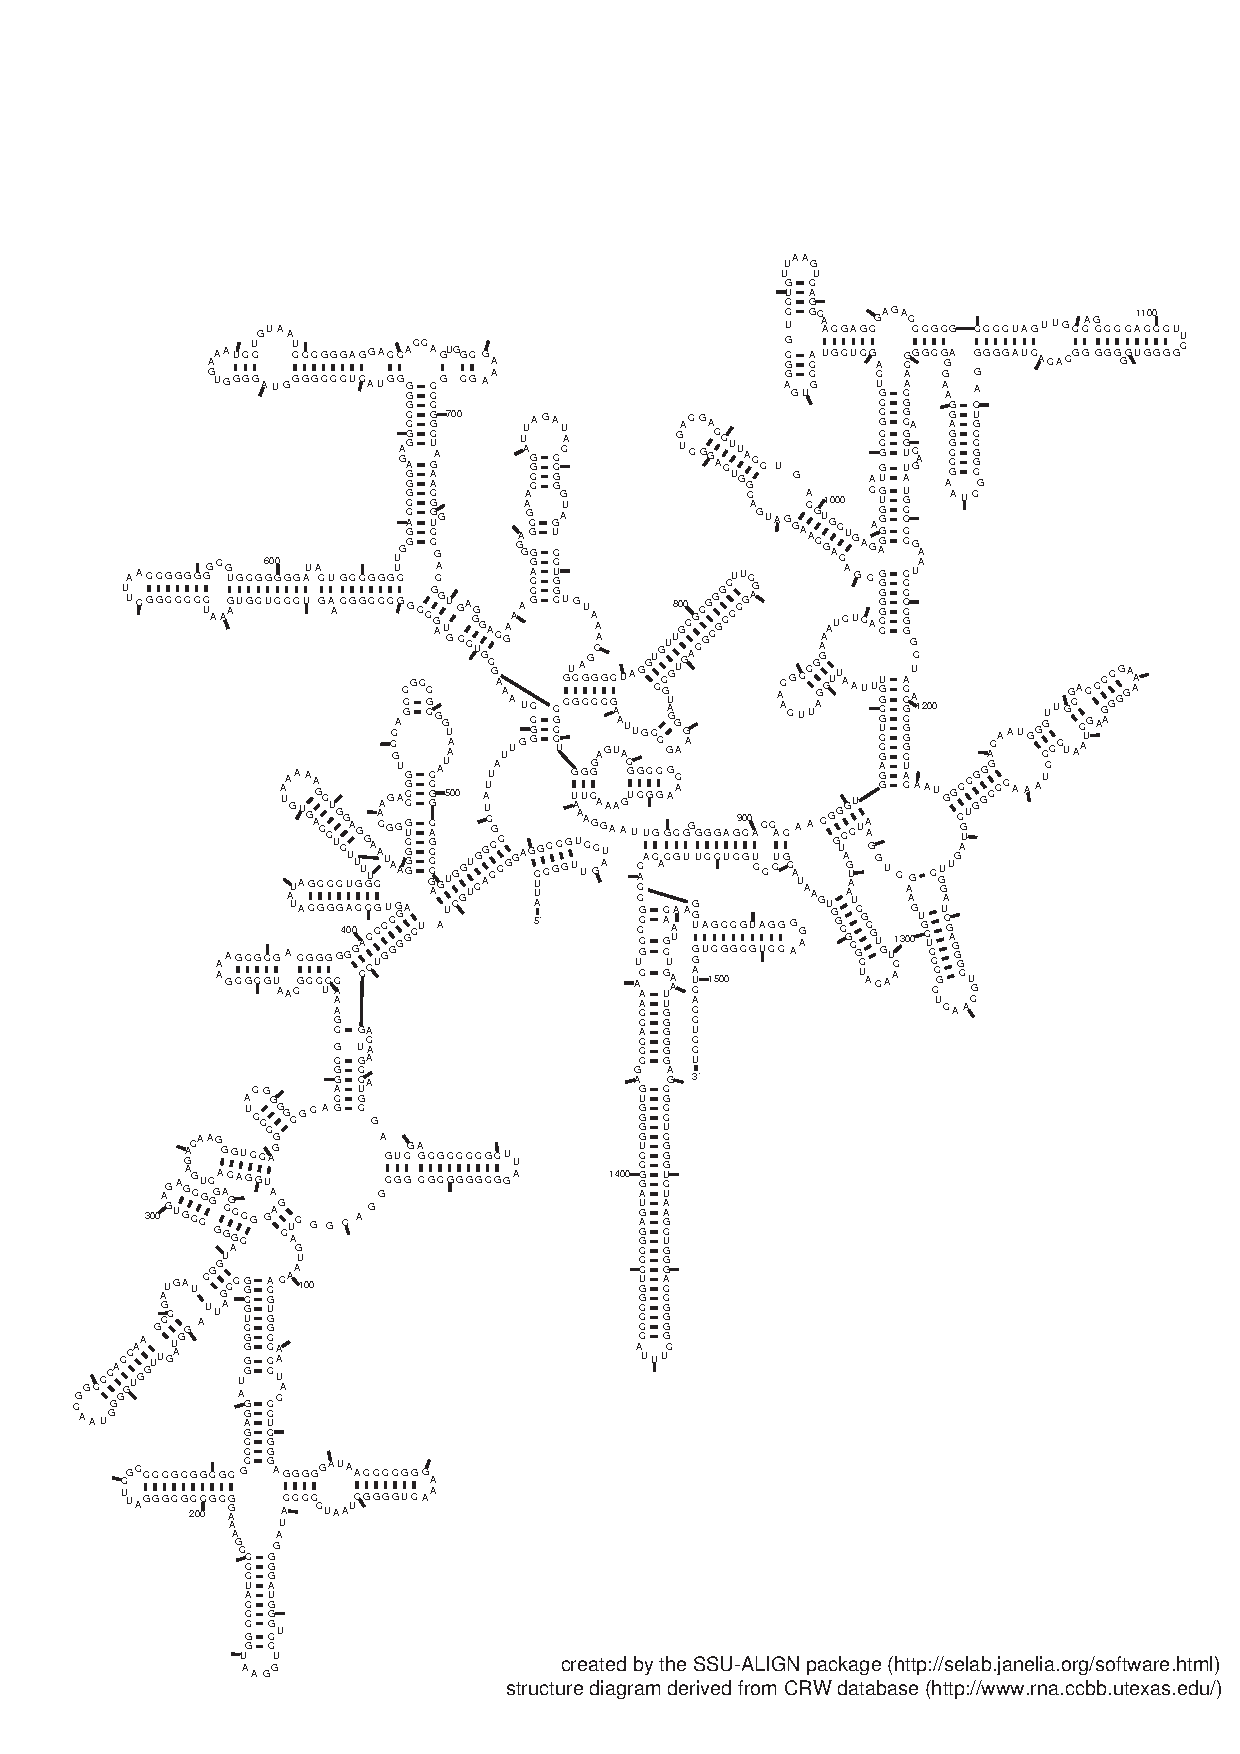
\includegraphics[height=8.5in]{../../seeds/ss-diagrams/archaea-0p1}

\newpage
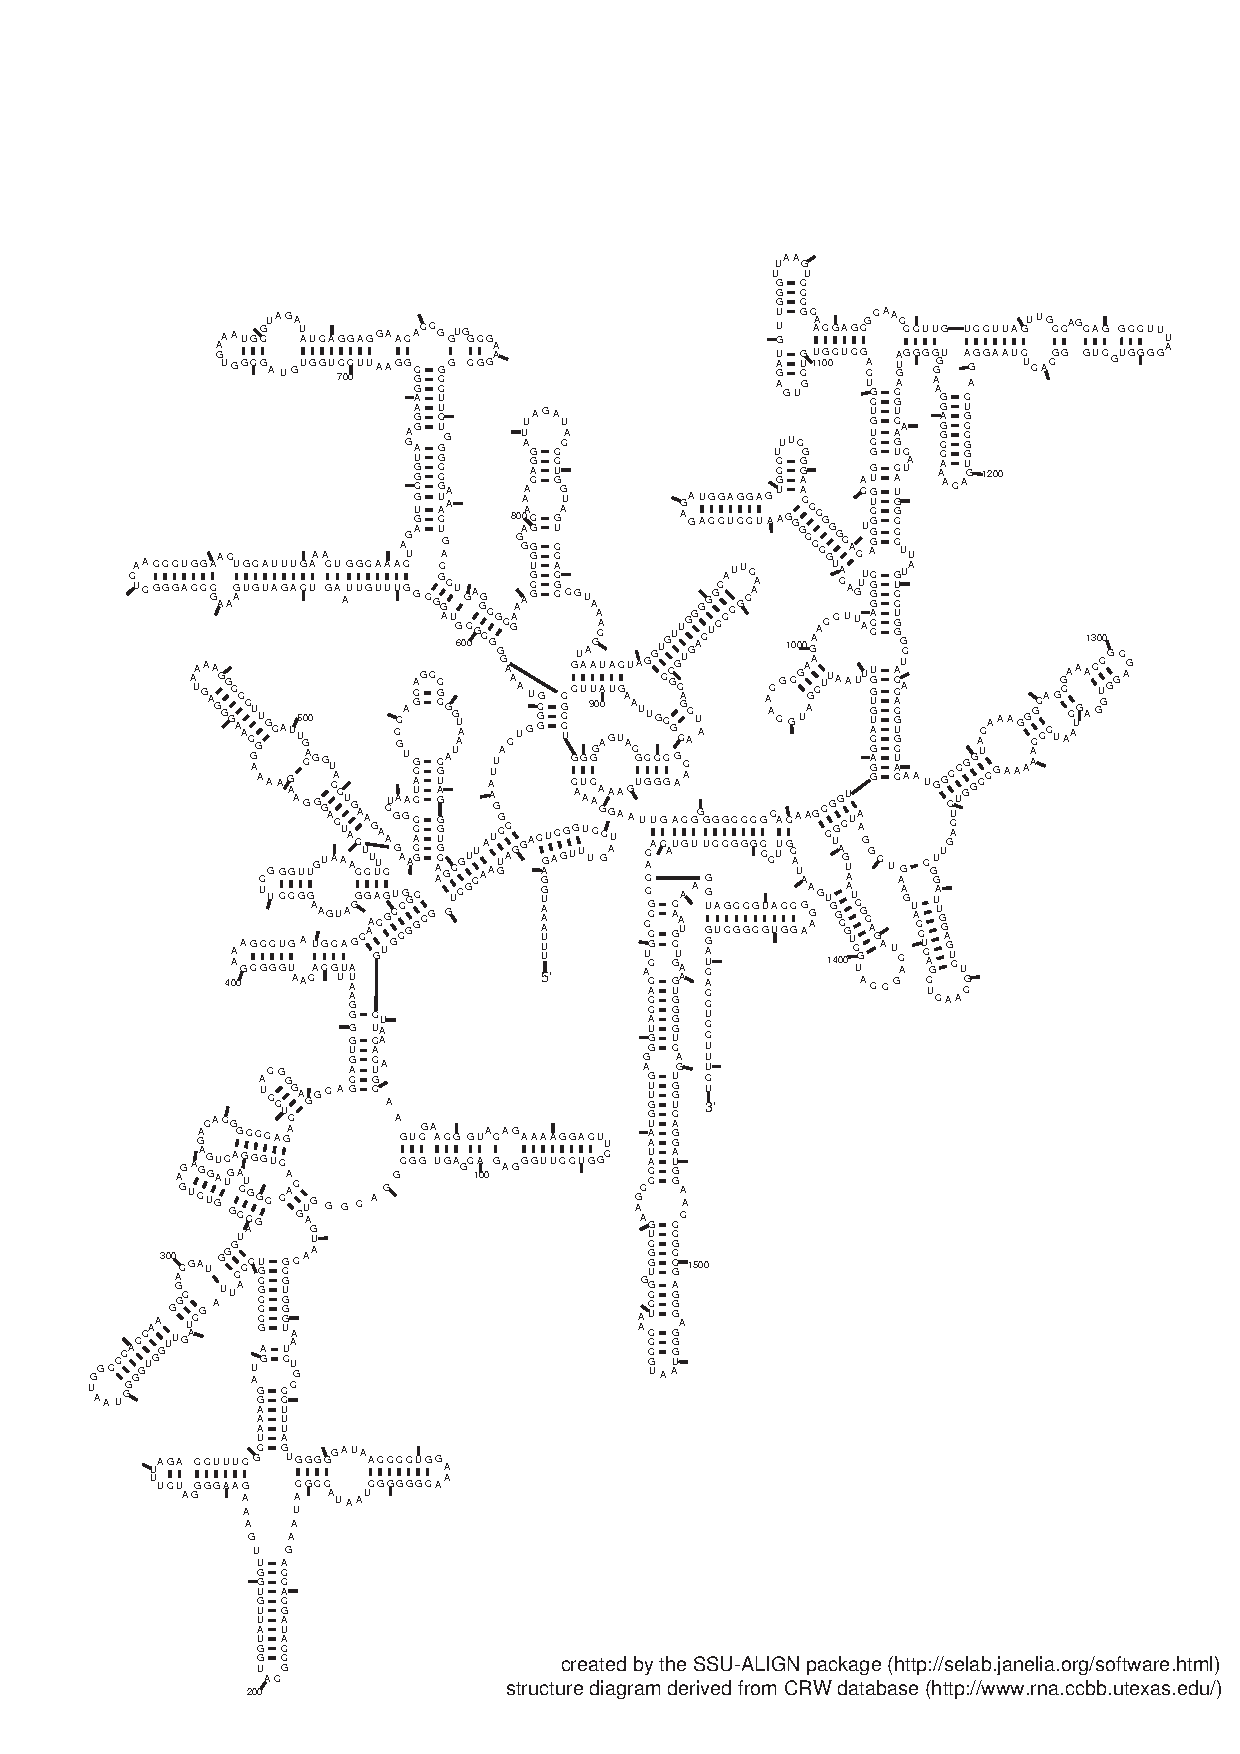
\includegraphics[height=8.5in]{../../seeds/ss-diagrams/bacteria-0p1}

\newpage
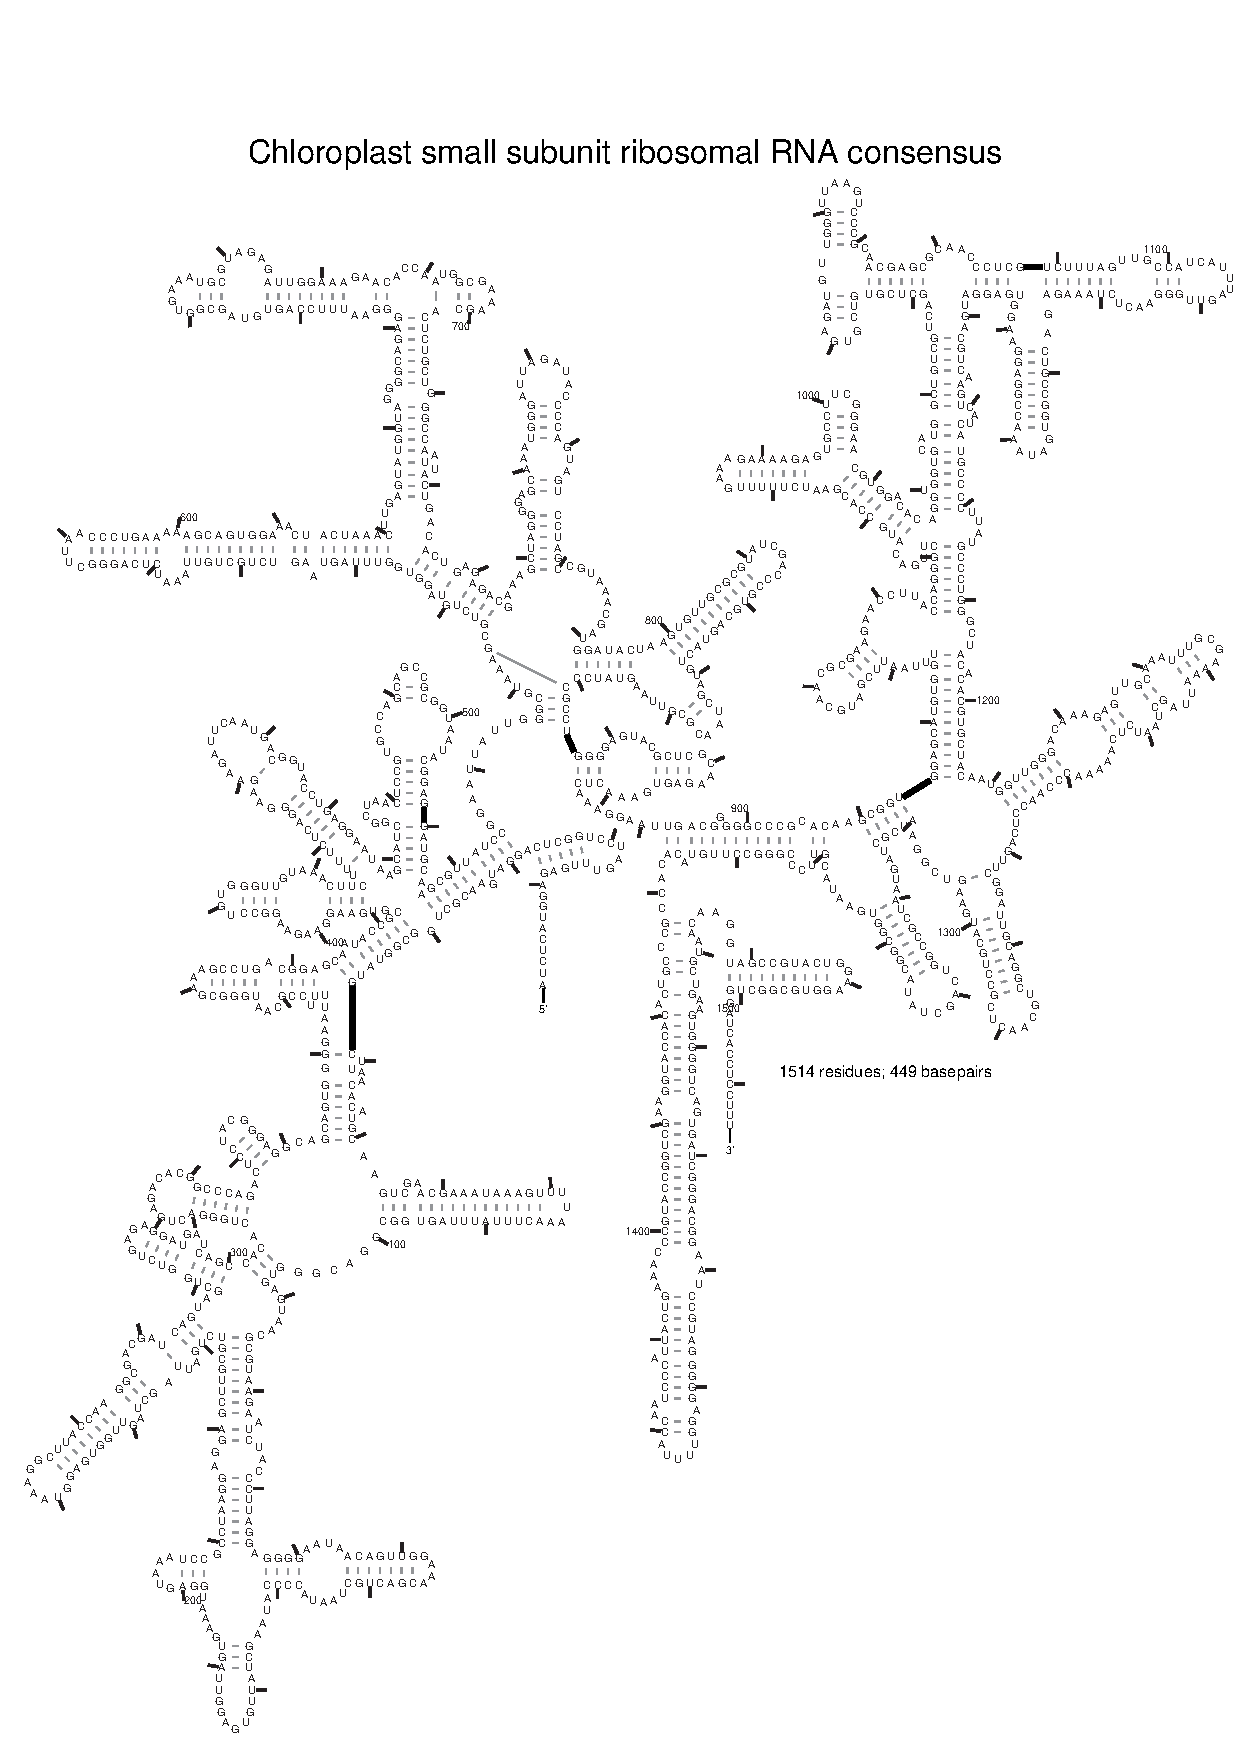
\includegraphics[height=8.5in]{../../seeds/ss-diagrams/chloroplast-0p1}

\newpage
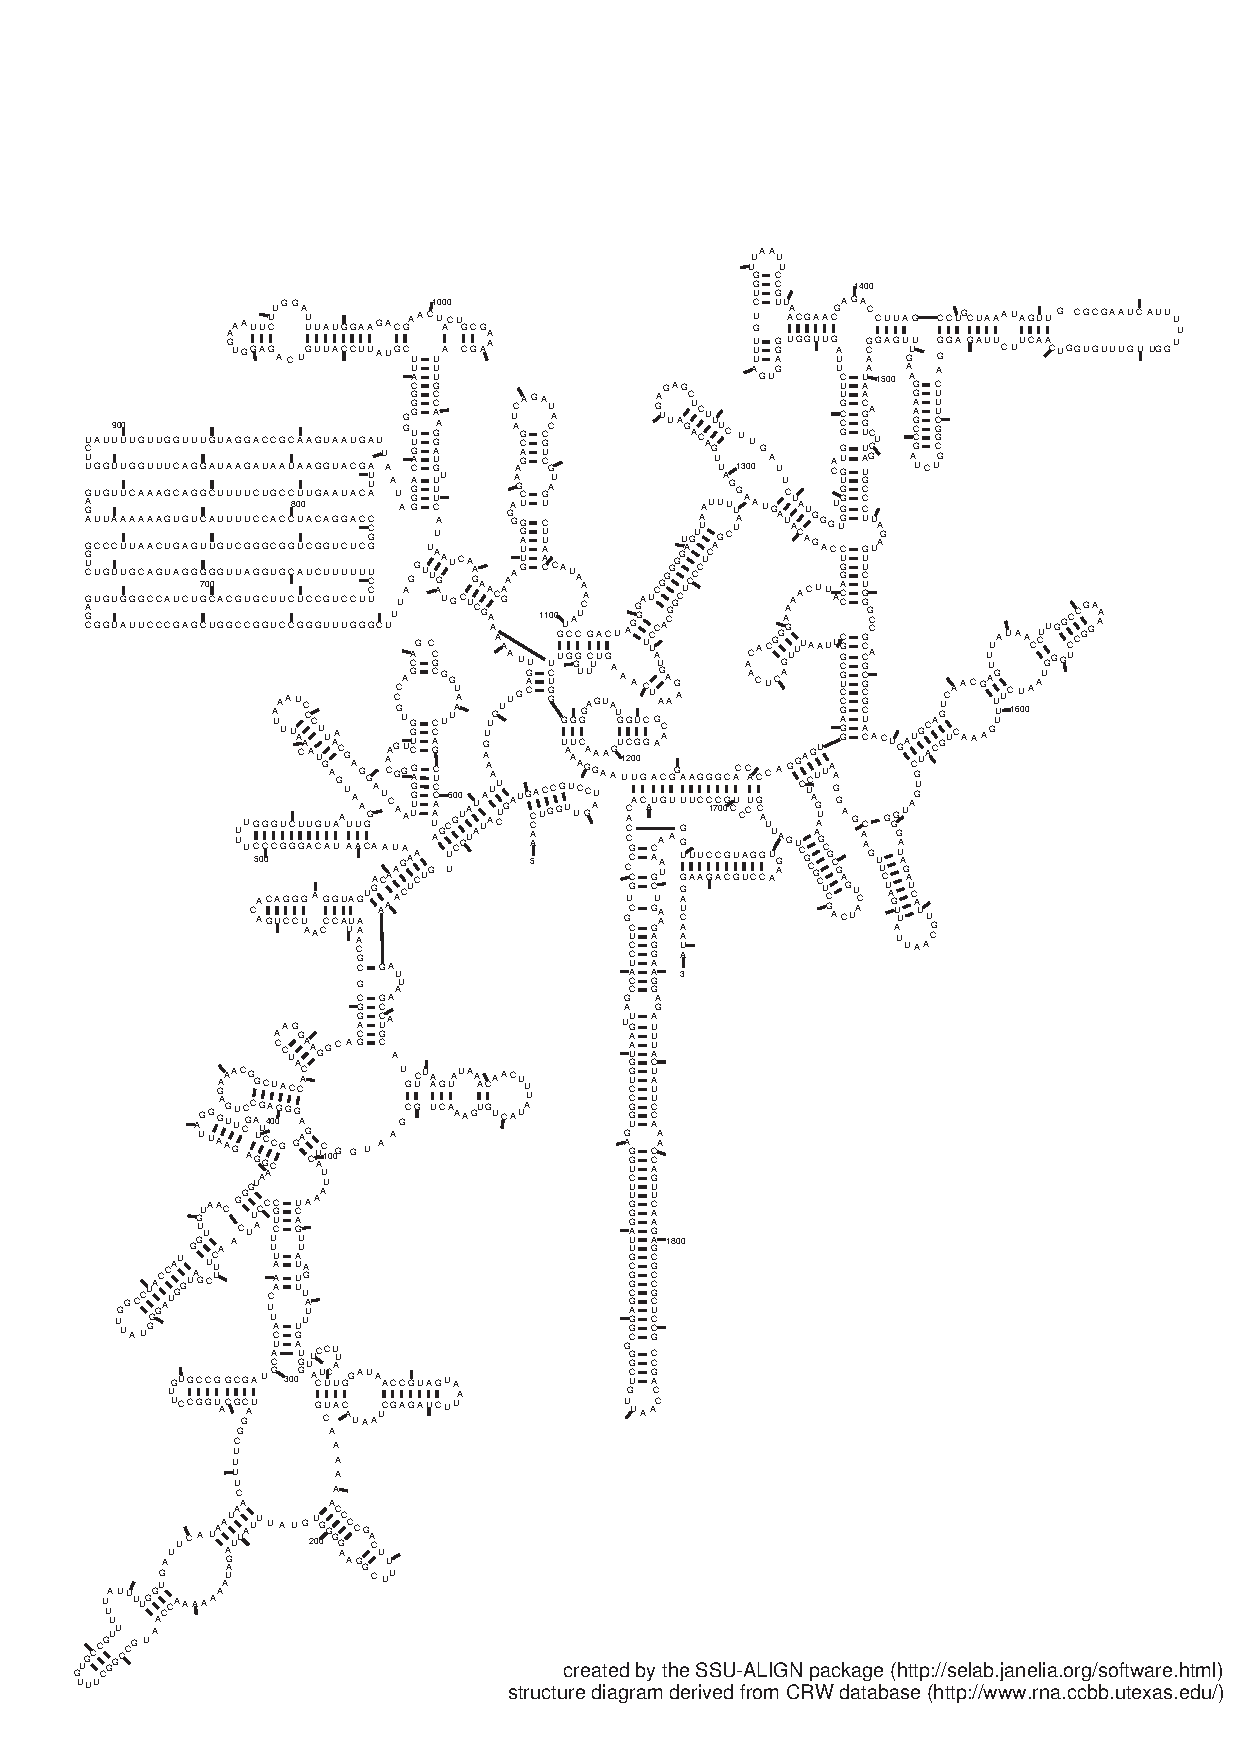
\includegraphics[height=8.5in]{../../seeds/ss-diagrams/eukarya-0p1}

\newpage
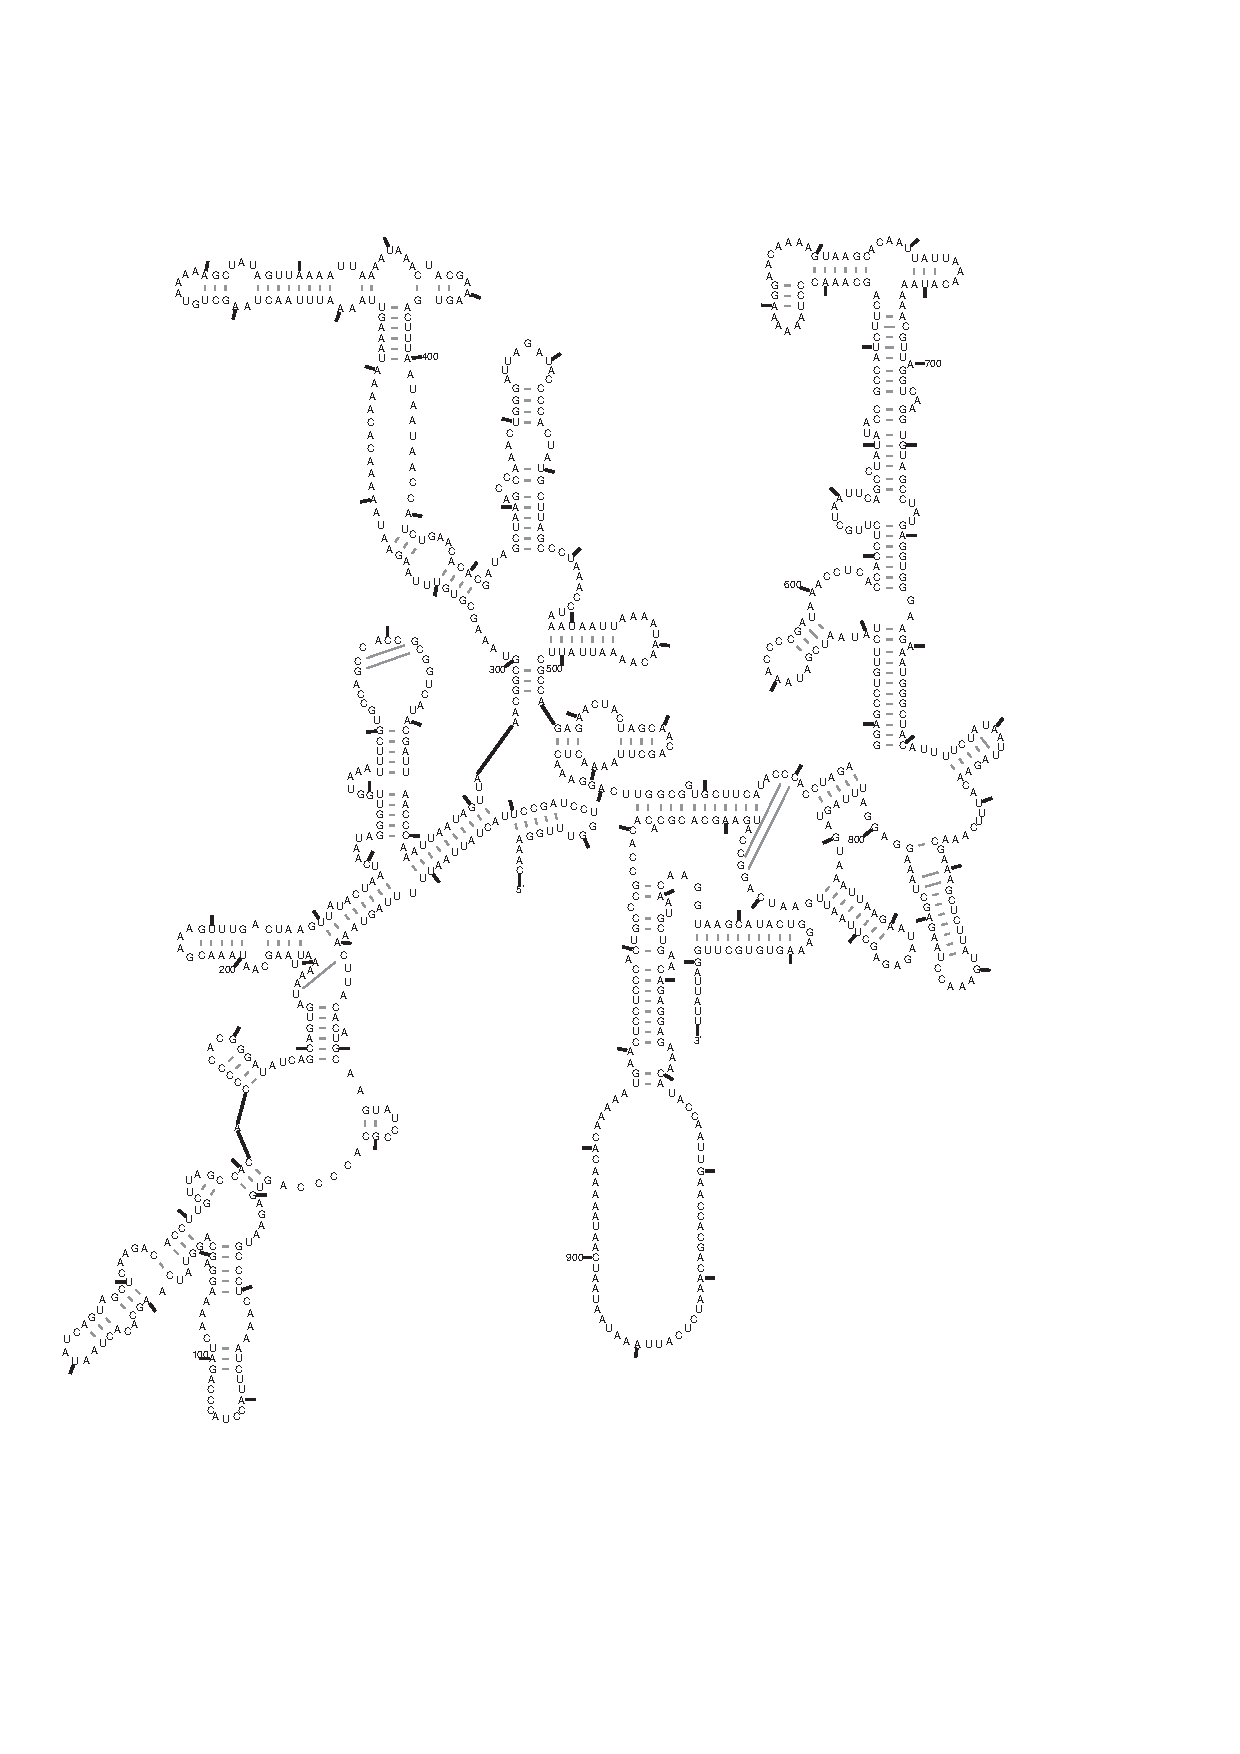
\includegraphics[height=8.5in]{../../seeds/ss-diagrams/metamito-0p1}

\end{center}

\begin{comment}
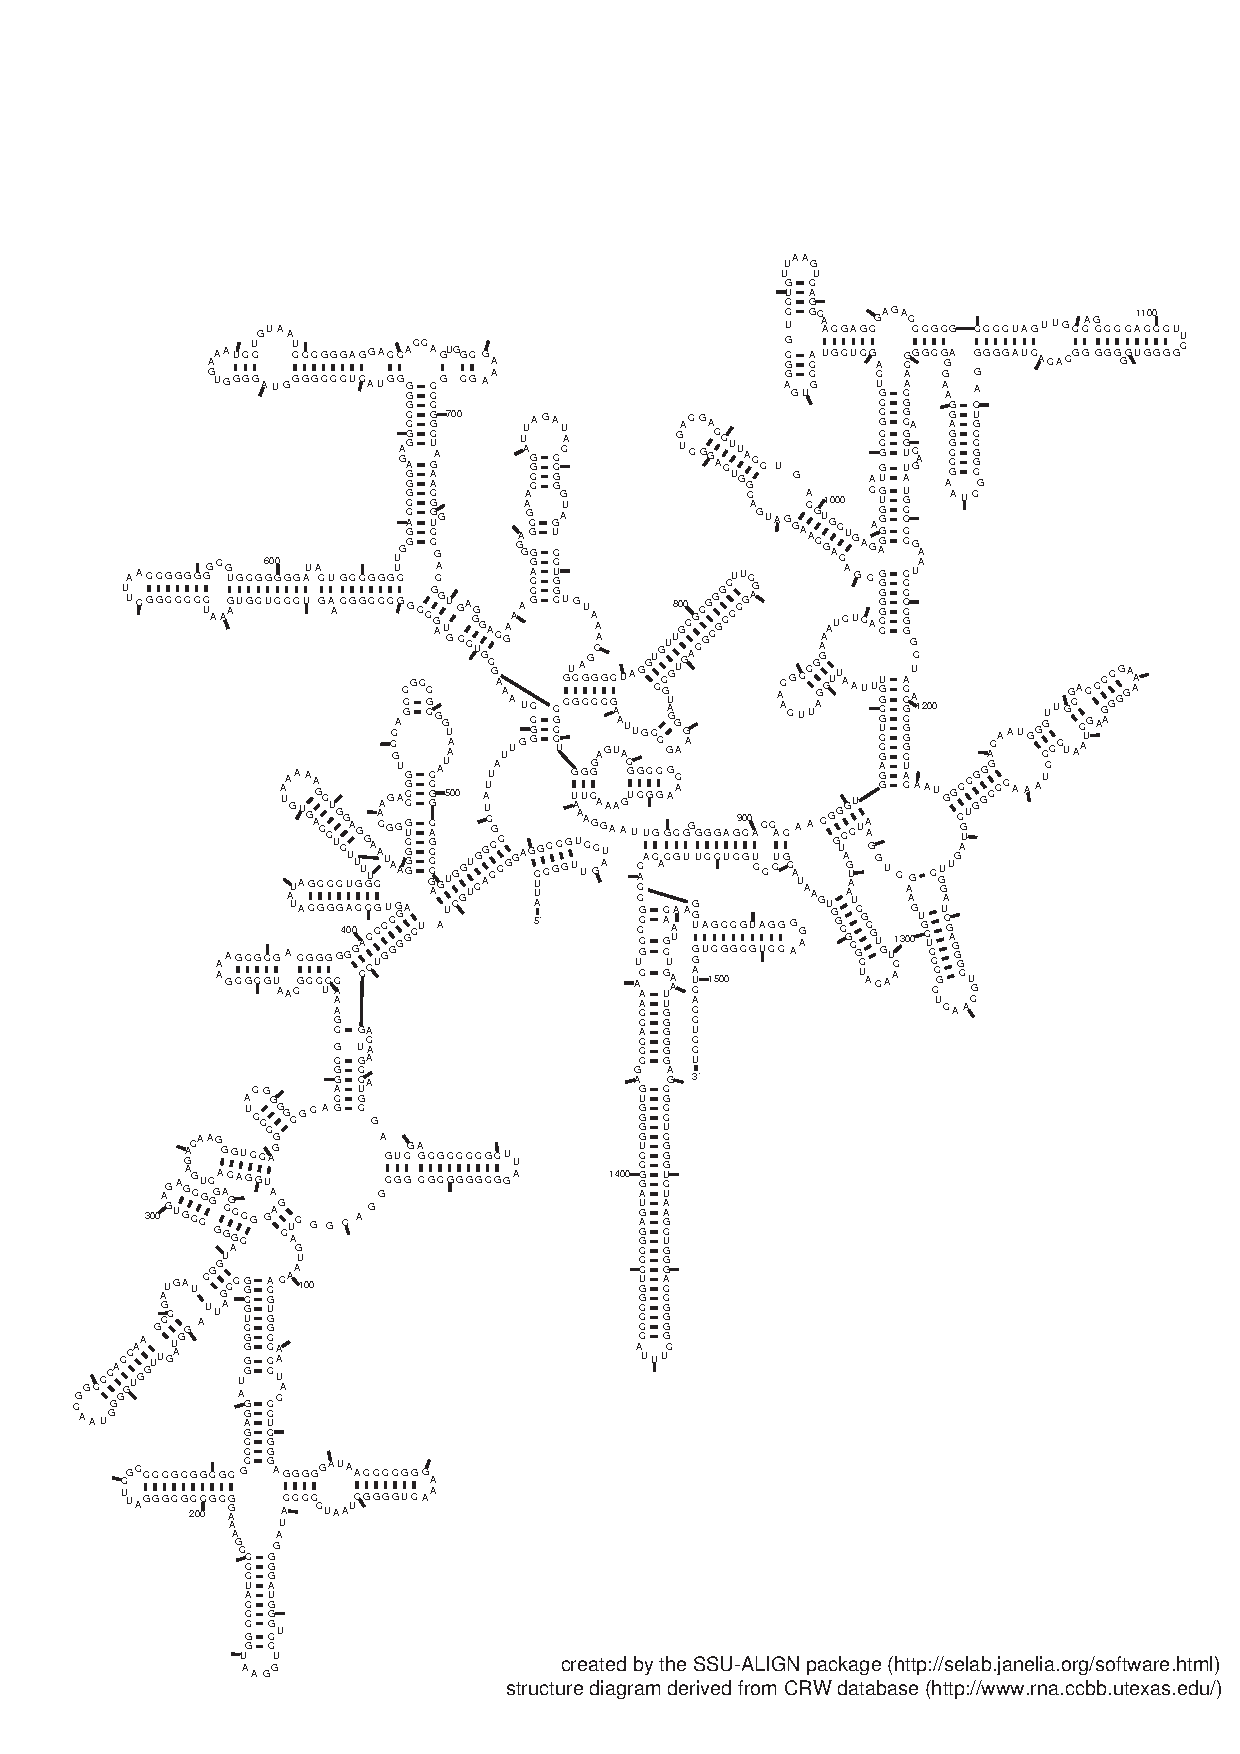
\includegraphics[height=8.5in]{../../seeds/ss-diagrams/archaea-0p1}
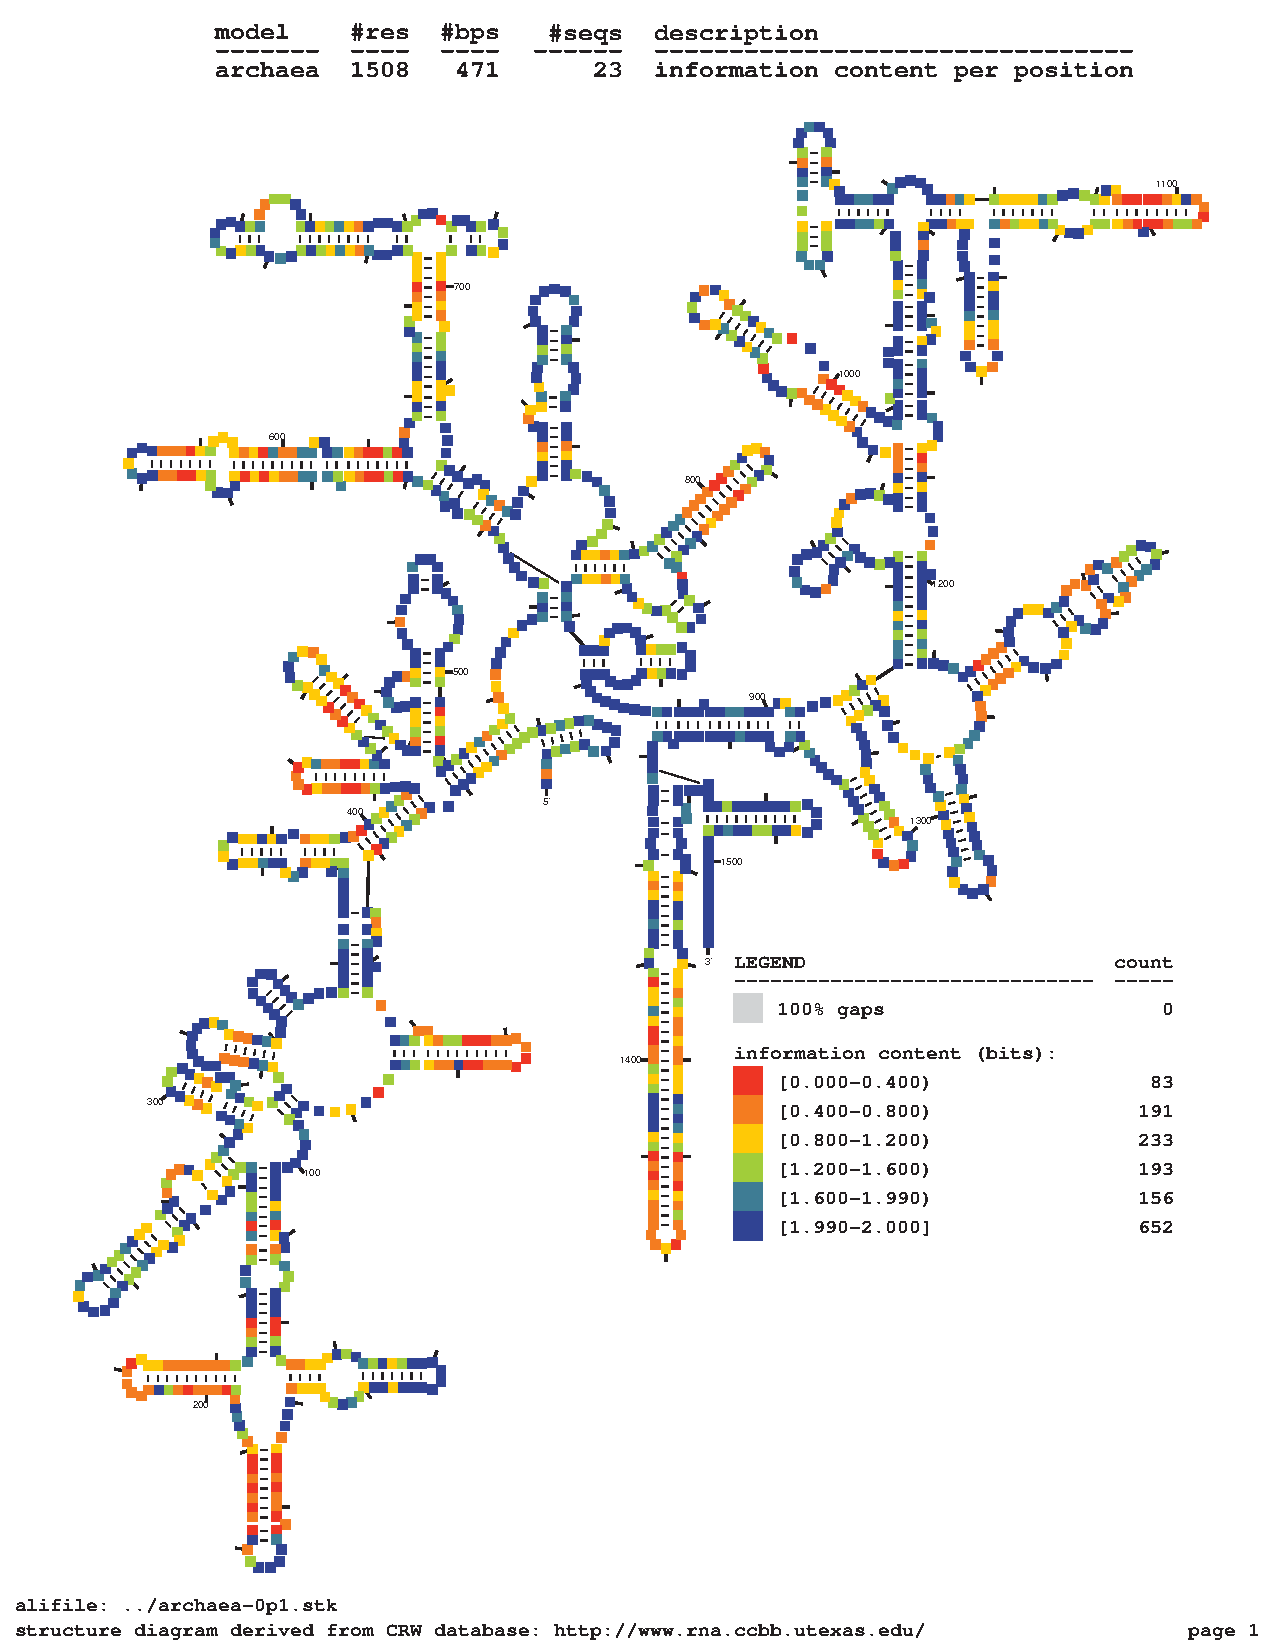
\includegraphics[height=8.5in]{../../seeds/ss-diagrams/archaea-0p1-info}
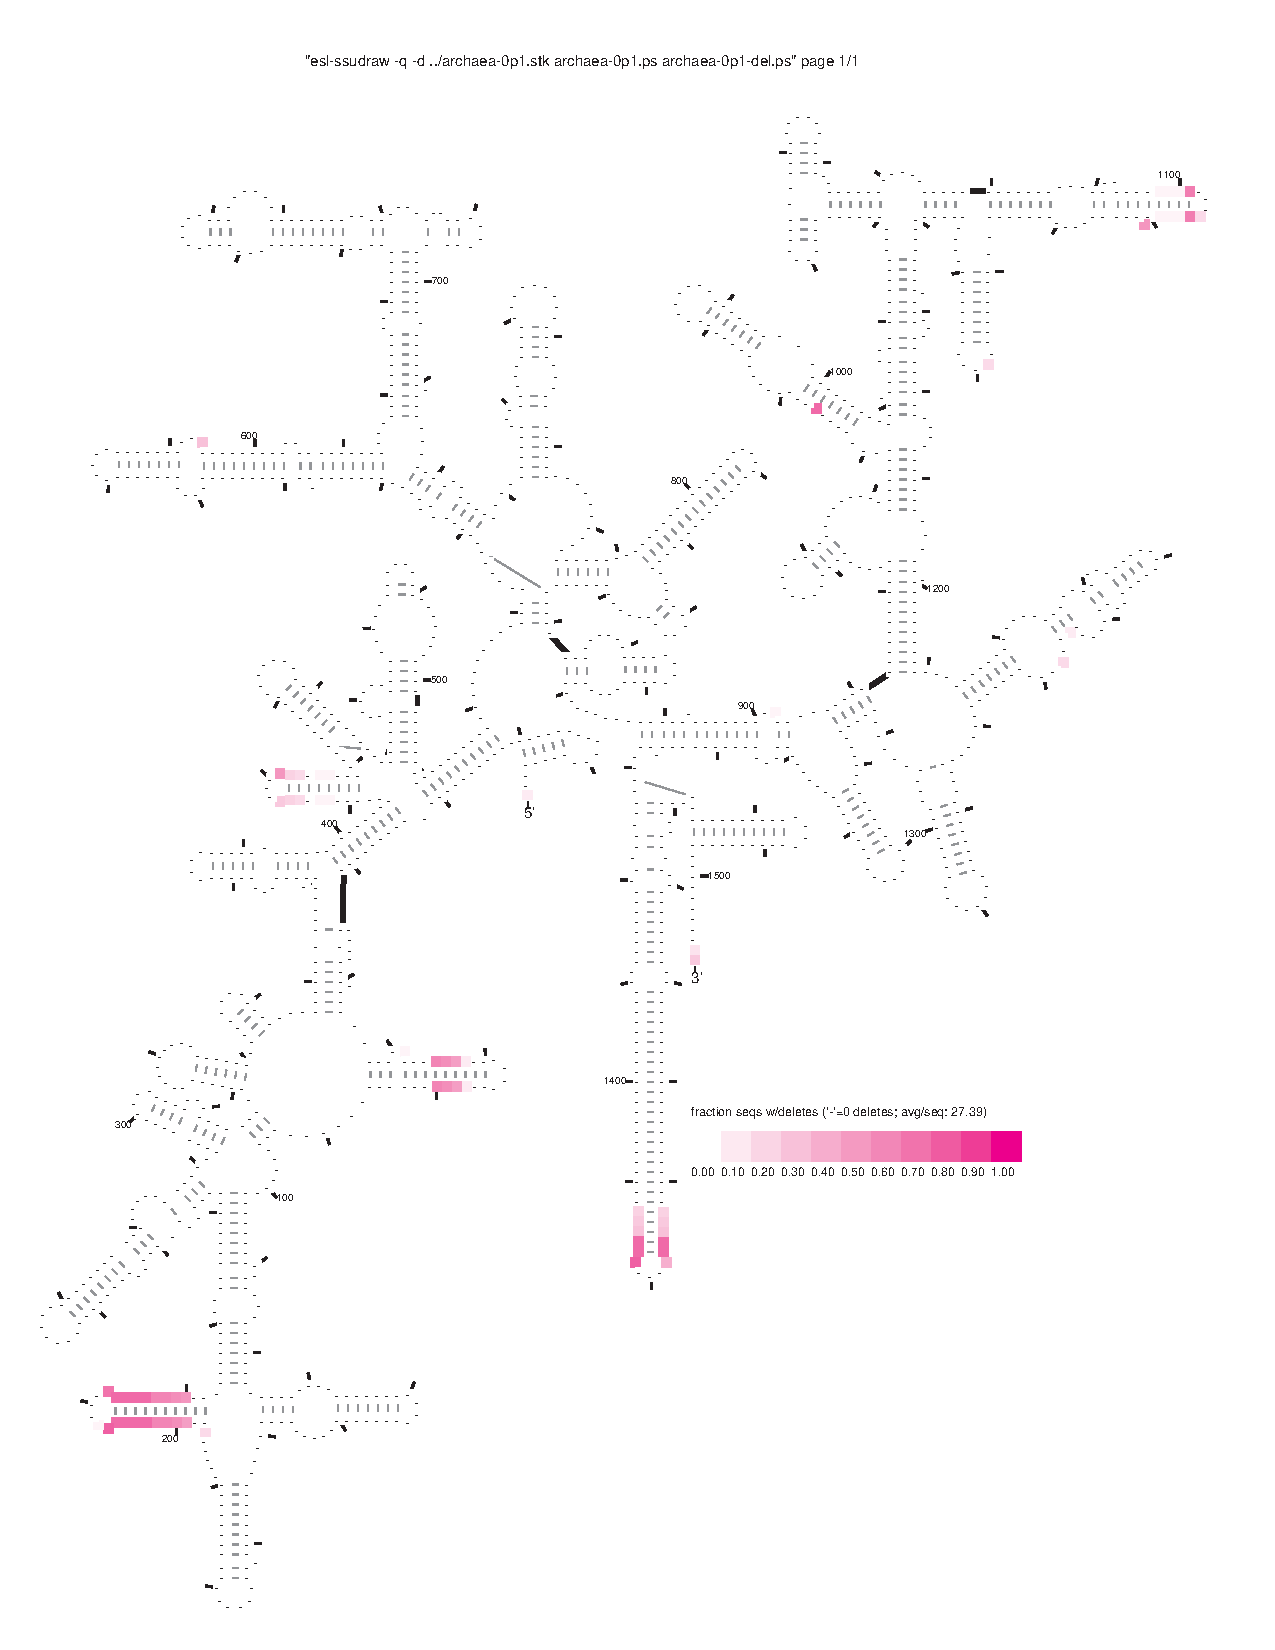
\includegraphics[height=8.5in]{../../seeds/ss-diagrams/archaea-0p1-del}
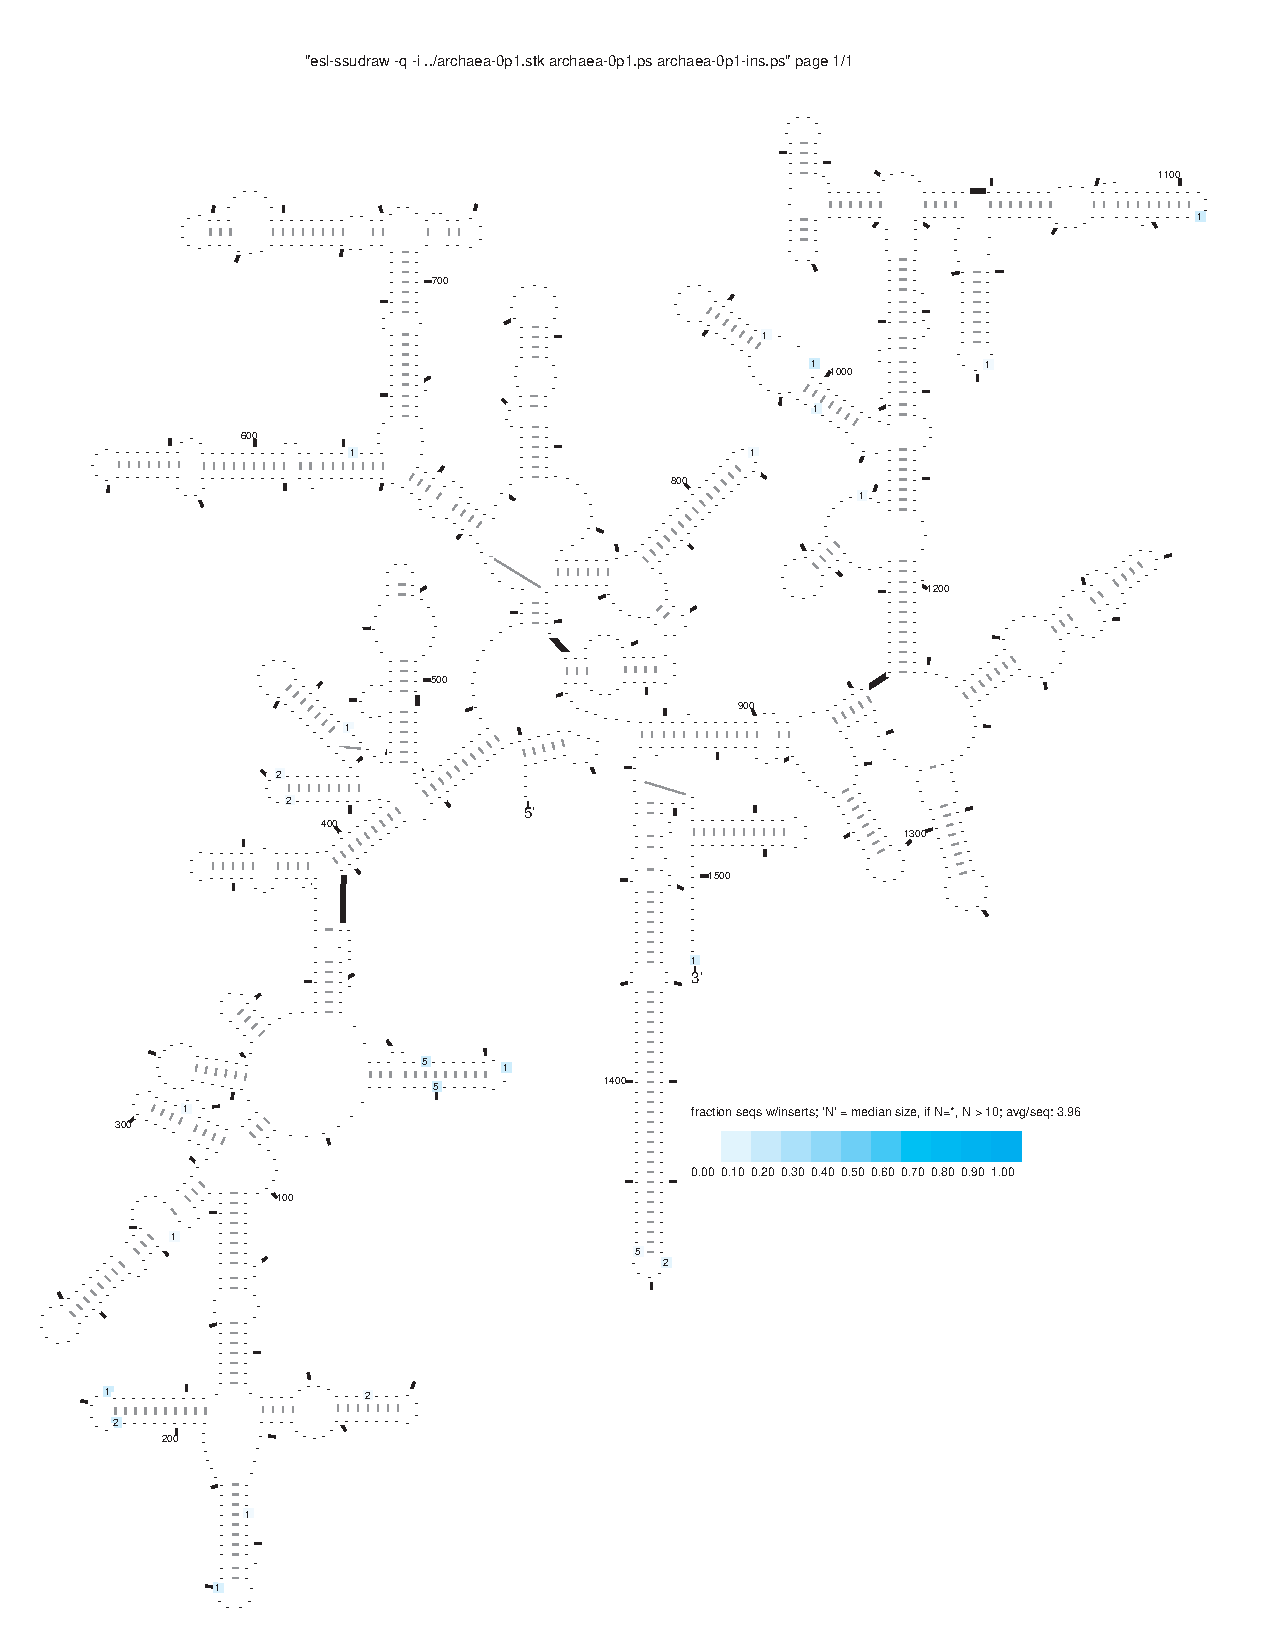
\includegraphics[height=8.5in]{../../seeds/ss-diagrams/archaea-0p1-ins}

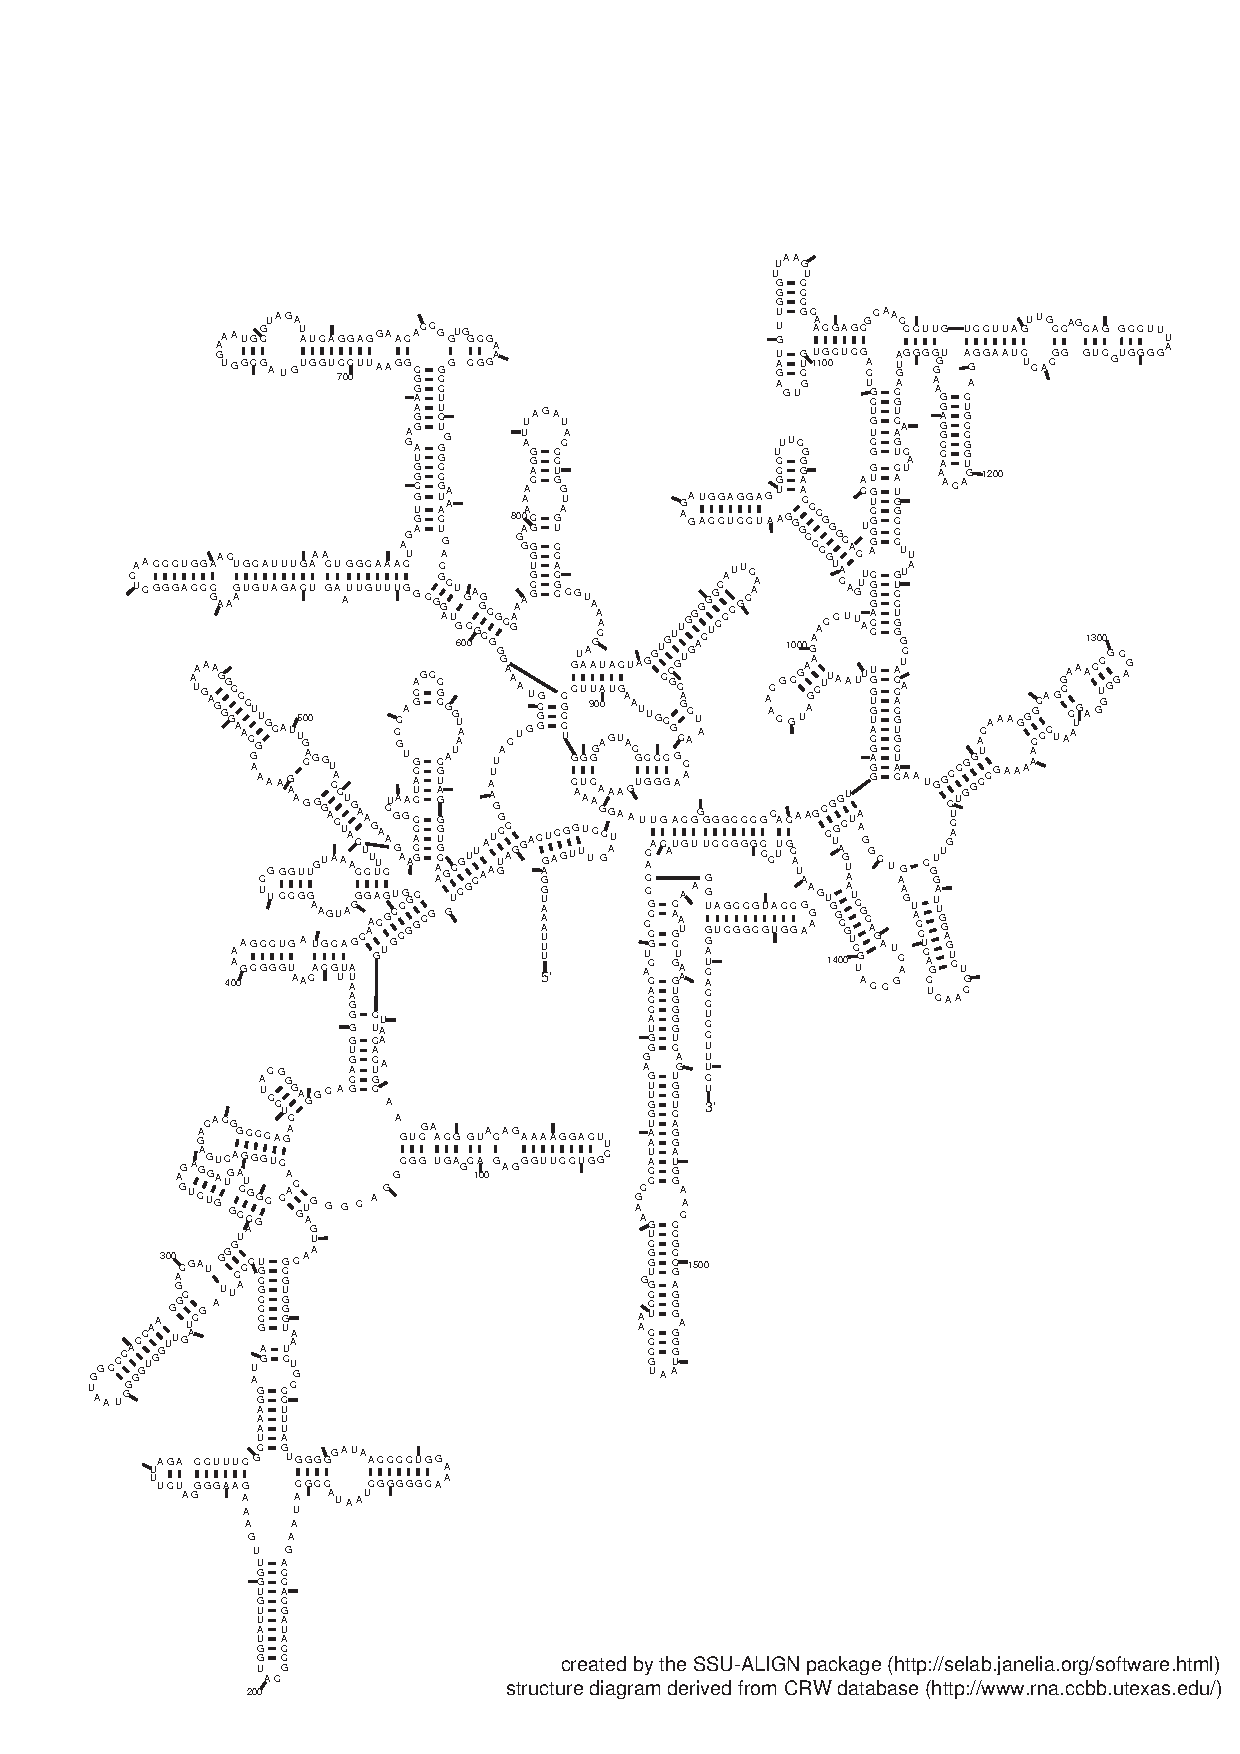
\includegraphics[height=8.5in]{../../seeds/ss-diagrams/bacteria-0p1}
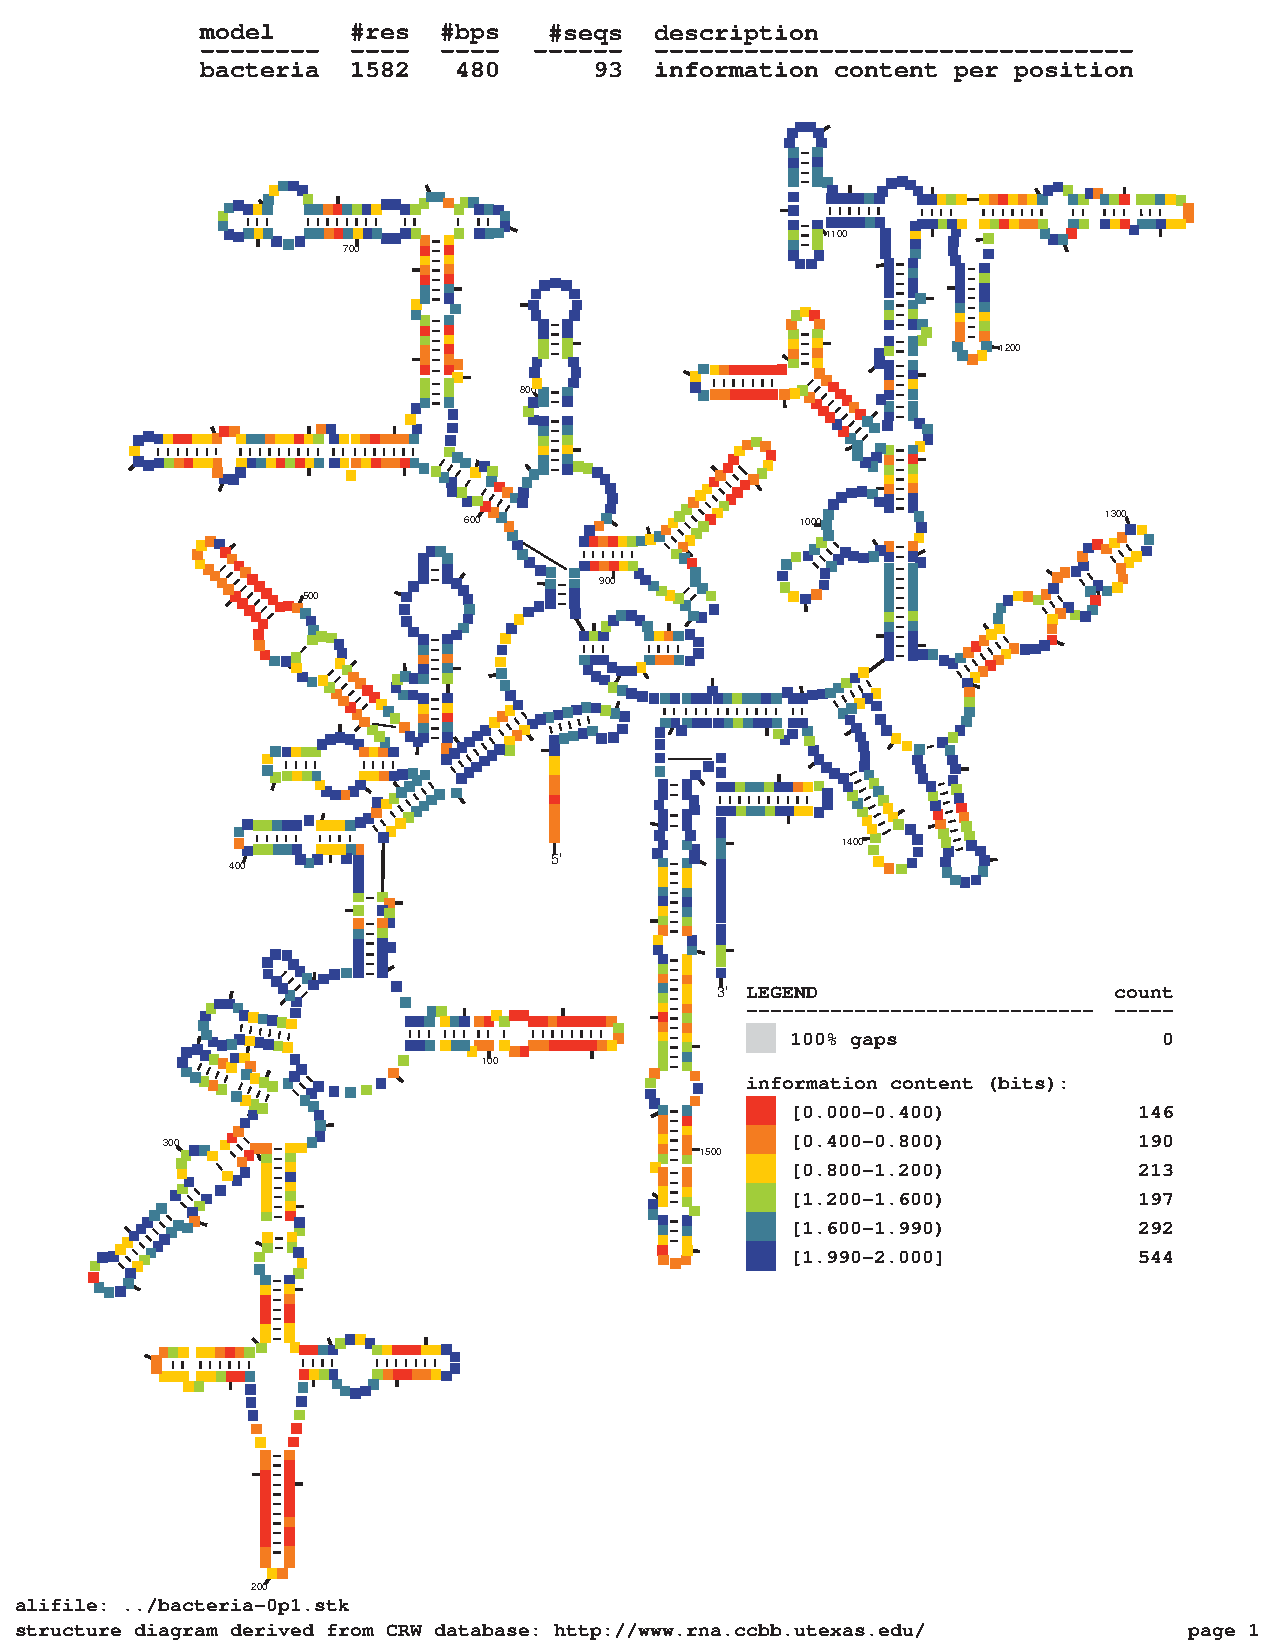
\includegraphics[height=8.5in]{../../seeds/ss-diagrams/bacteria-0p1-info}
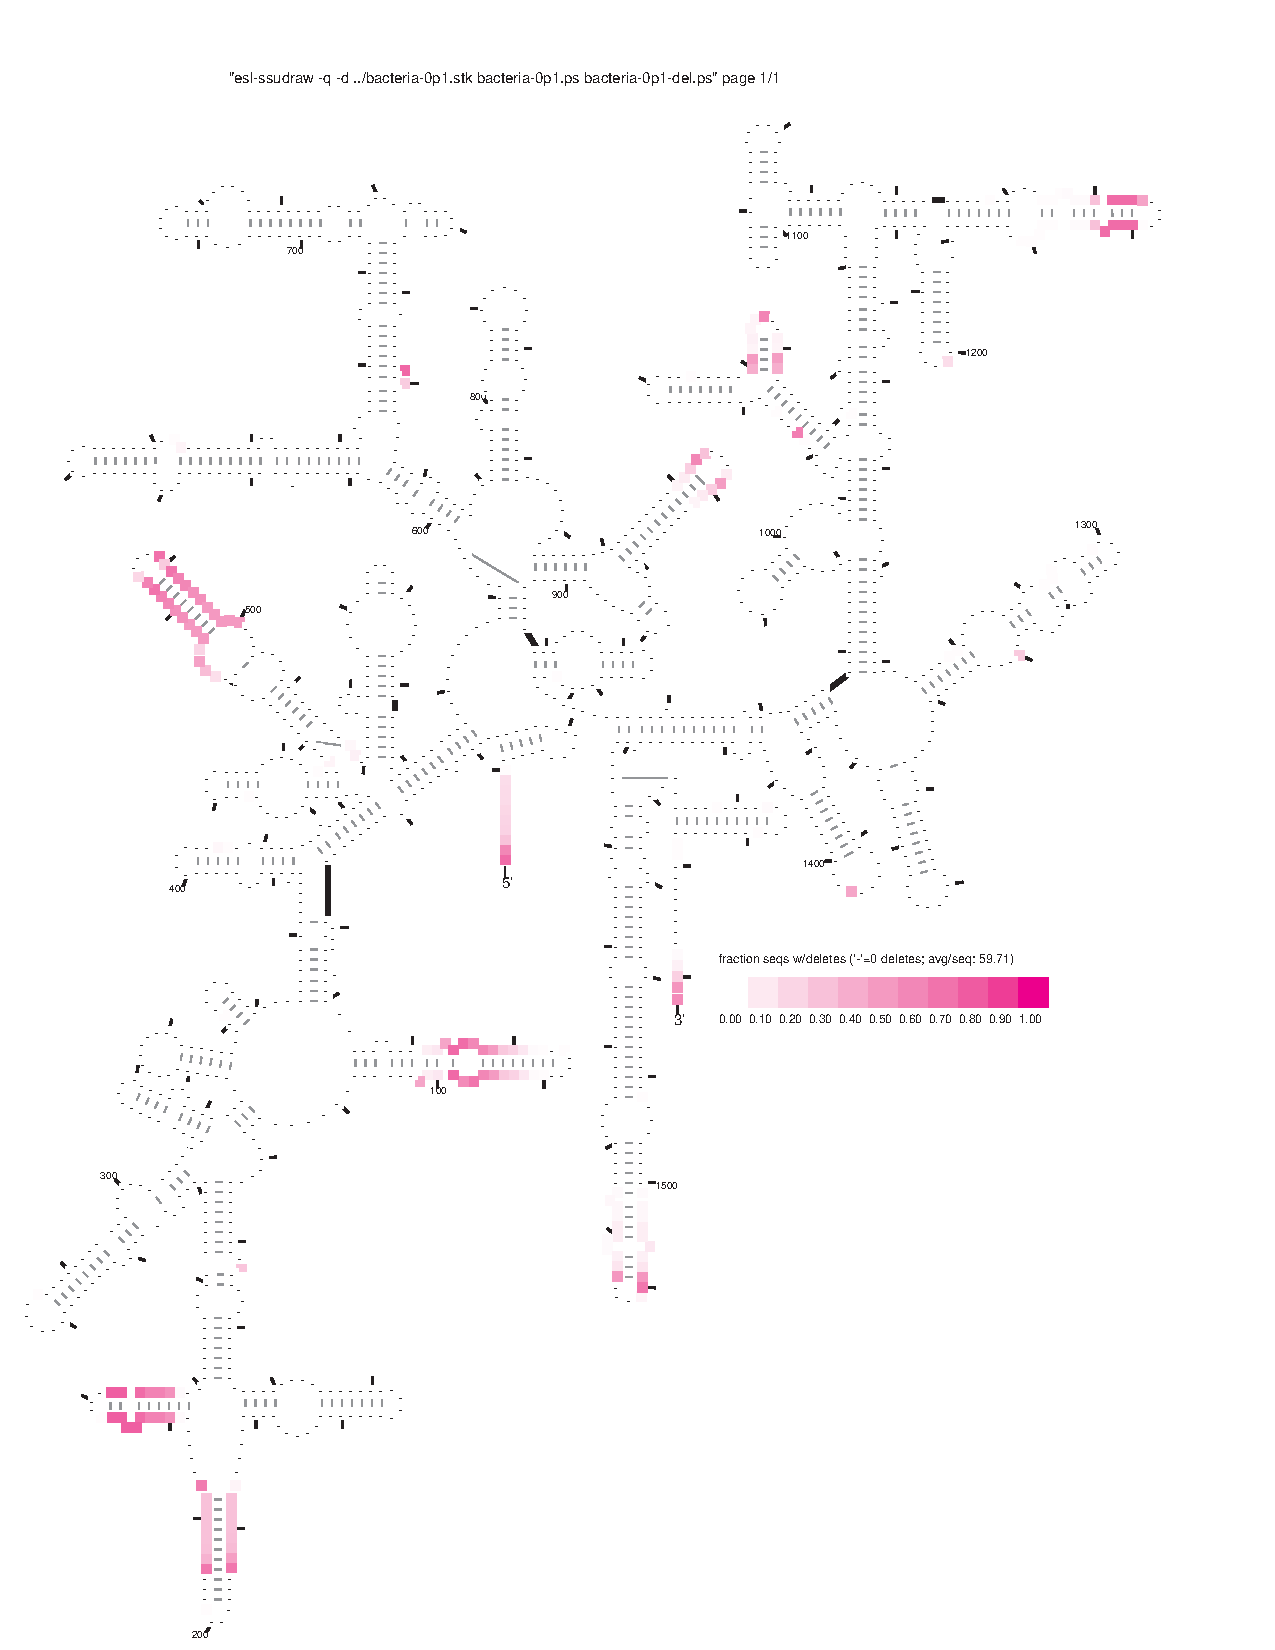
\includegraphics[height=8.5in]{../../seeds/ss-diagrams/bacteria-0p1-del}
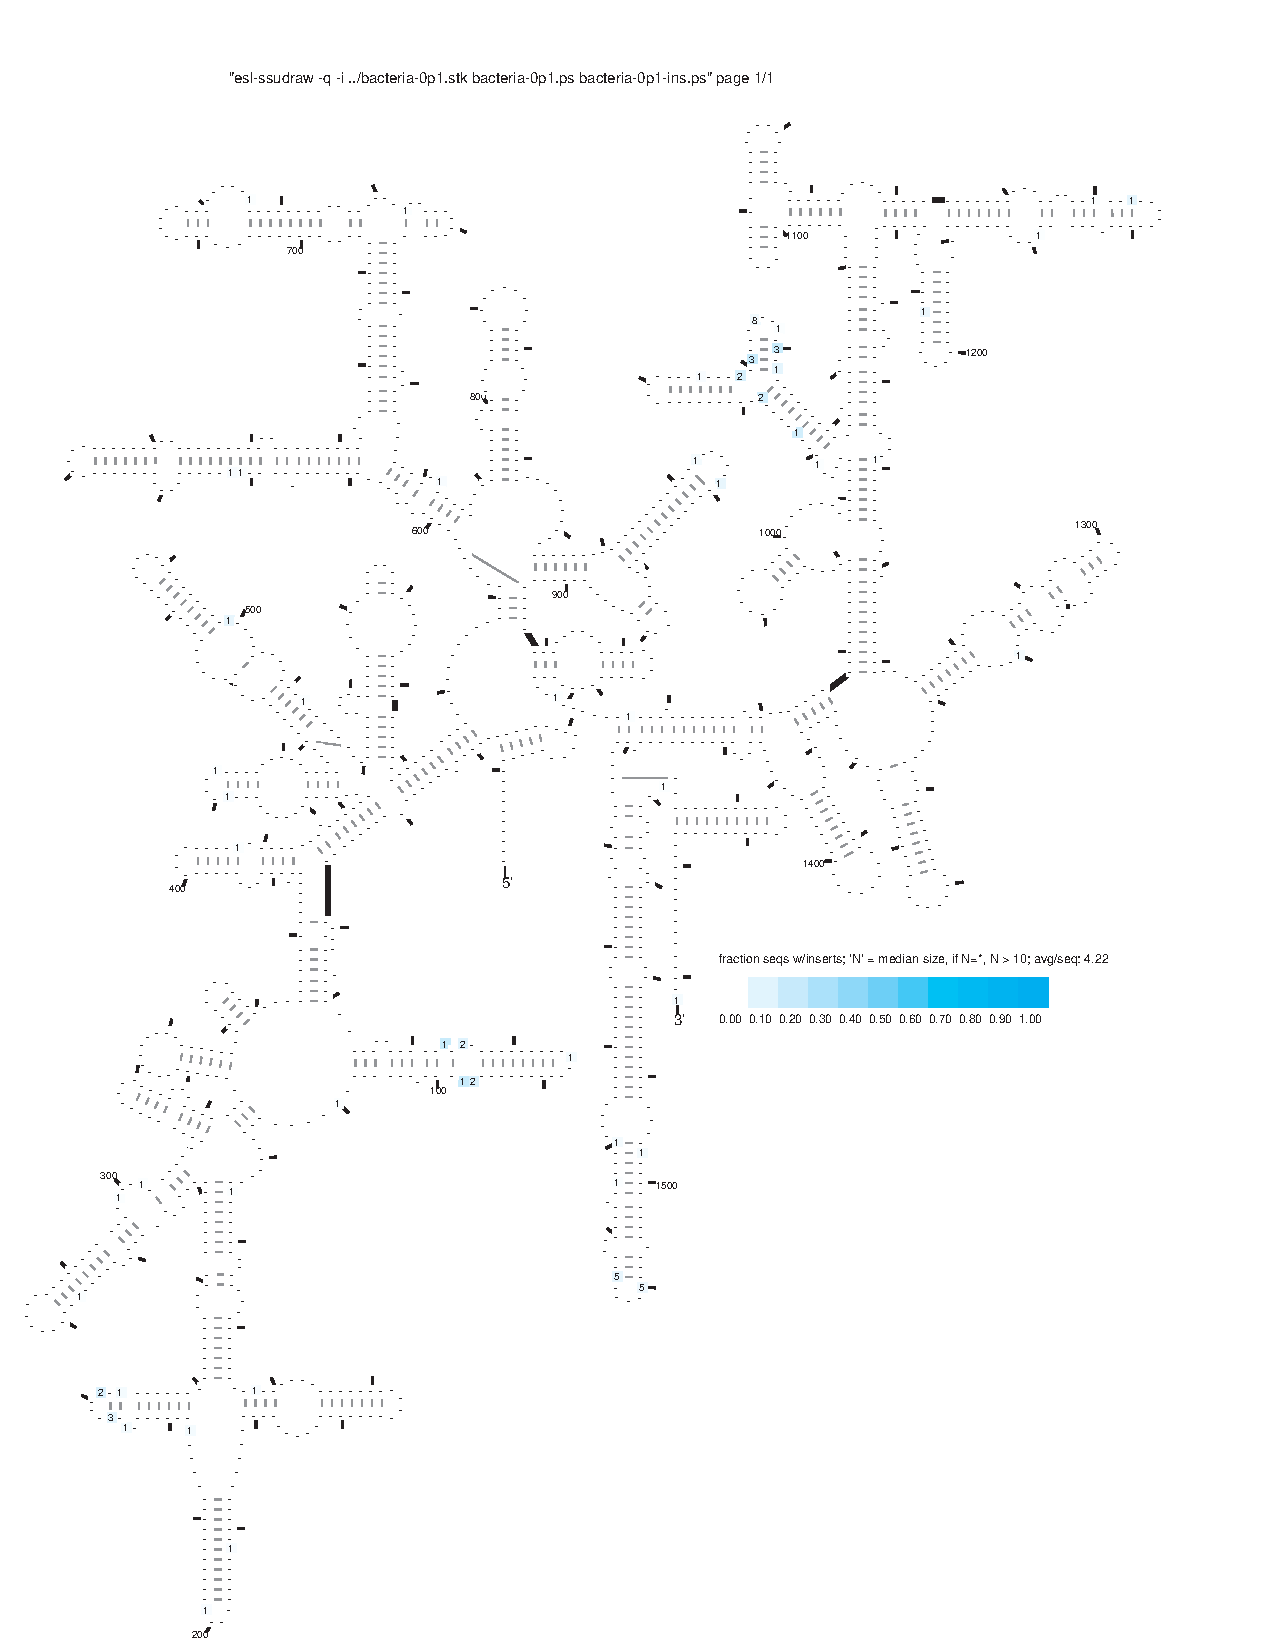
\includegraphics[height=8.5in]{../../seeds/ss-diagrams/bacteria-0p1-ins}

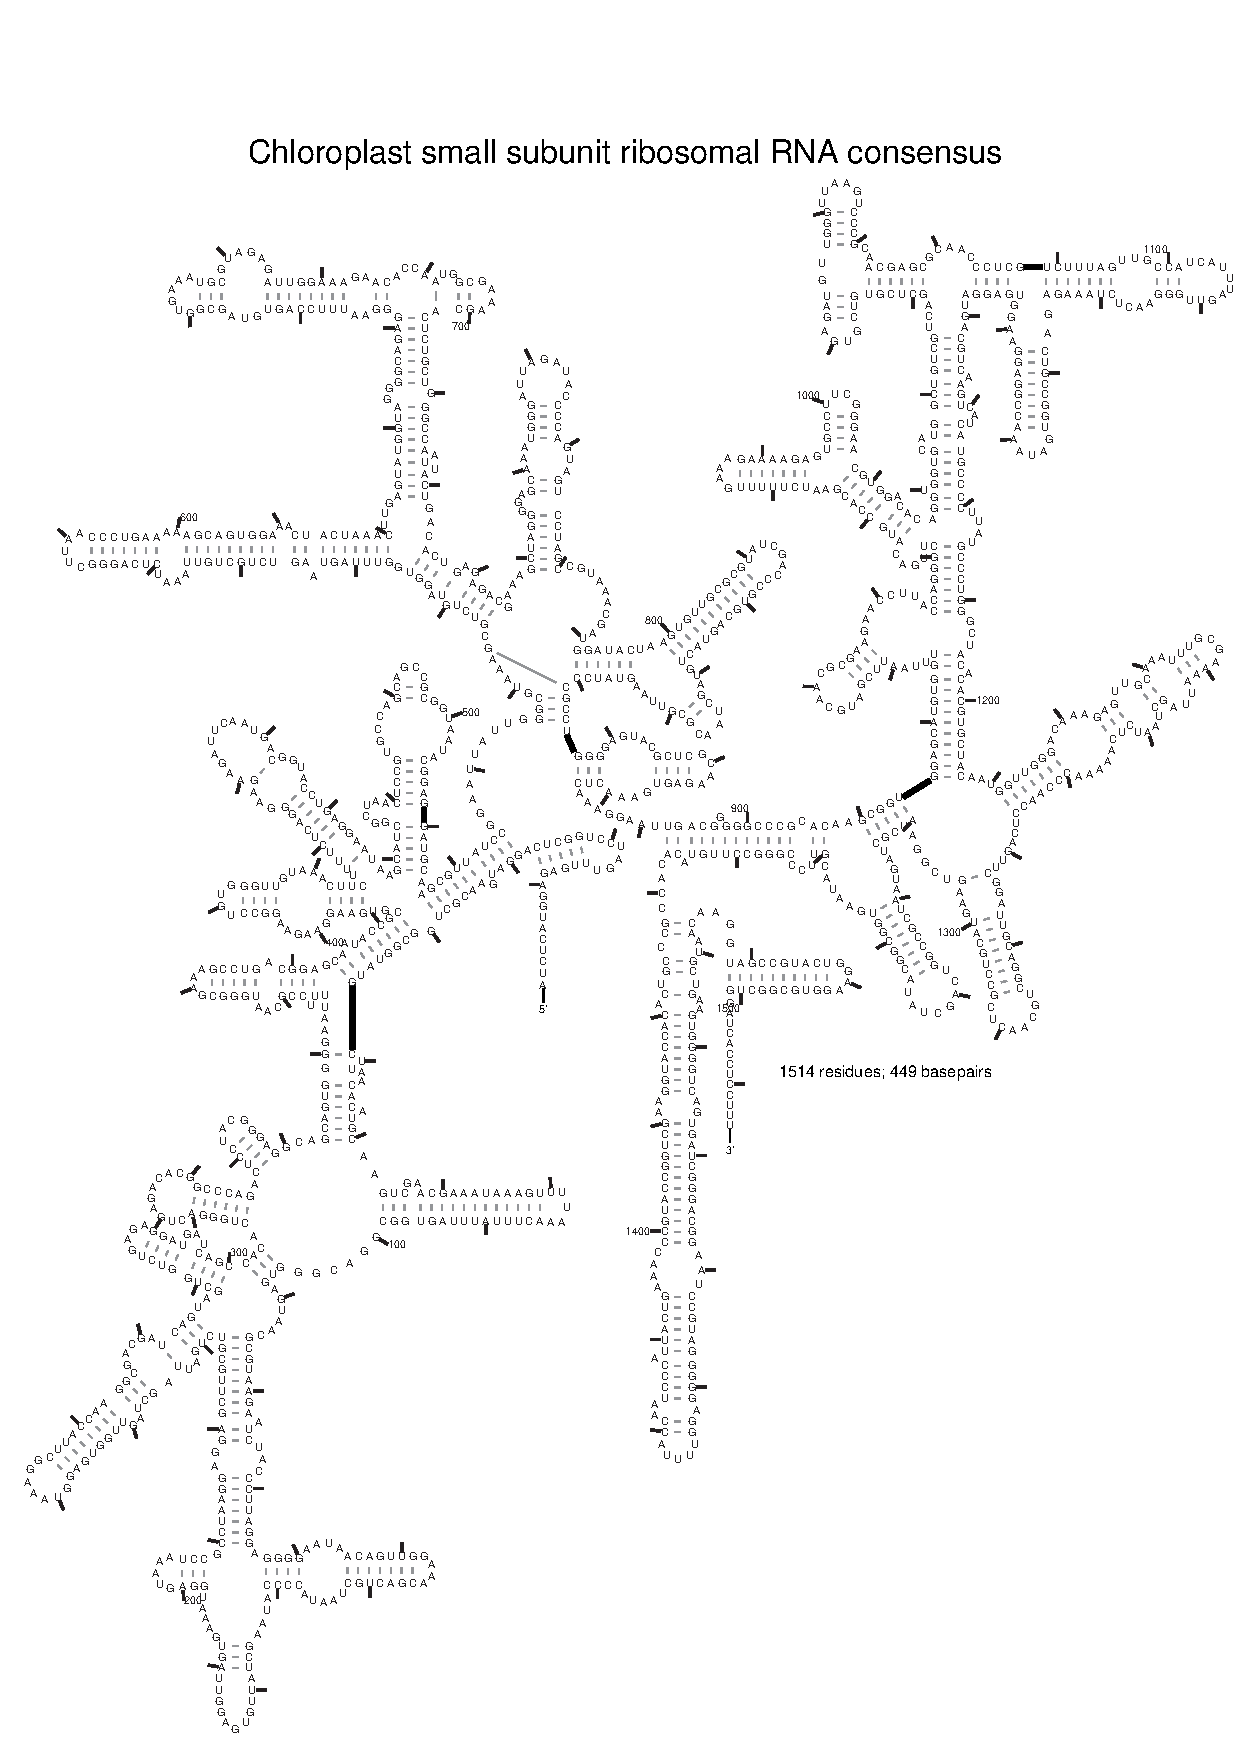
\includegraphics[height=8.5in]{../../seeds/ss-diagrams/chloroplast-0p1}
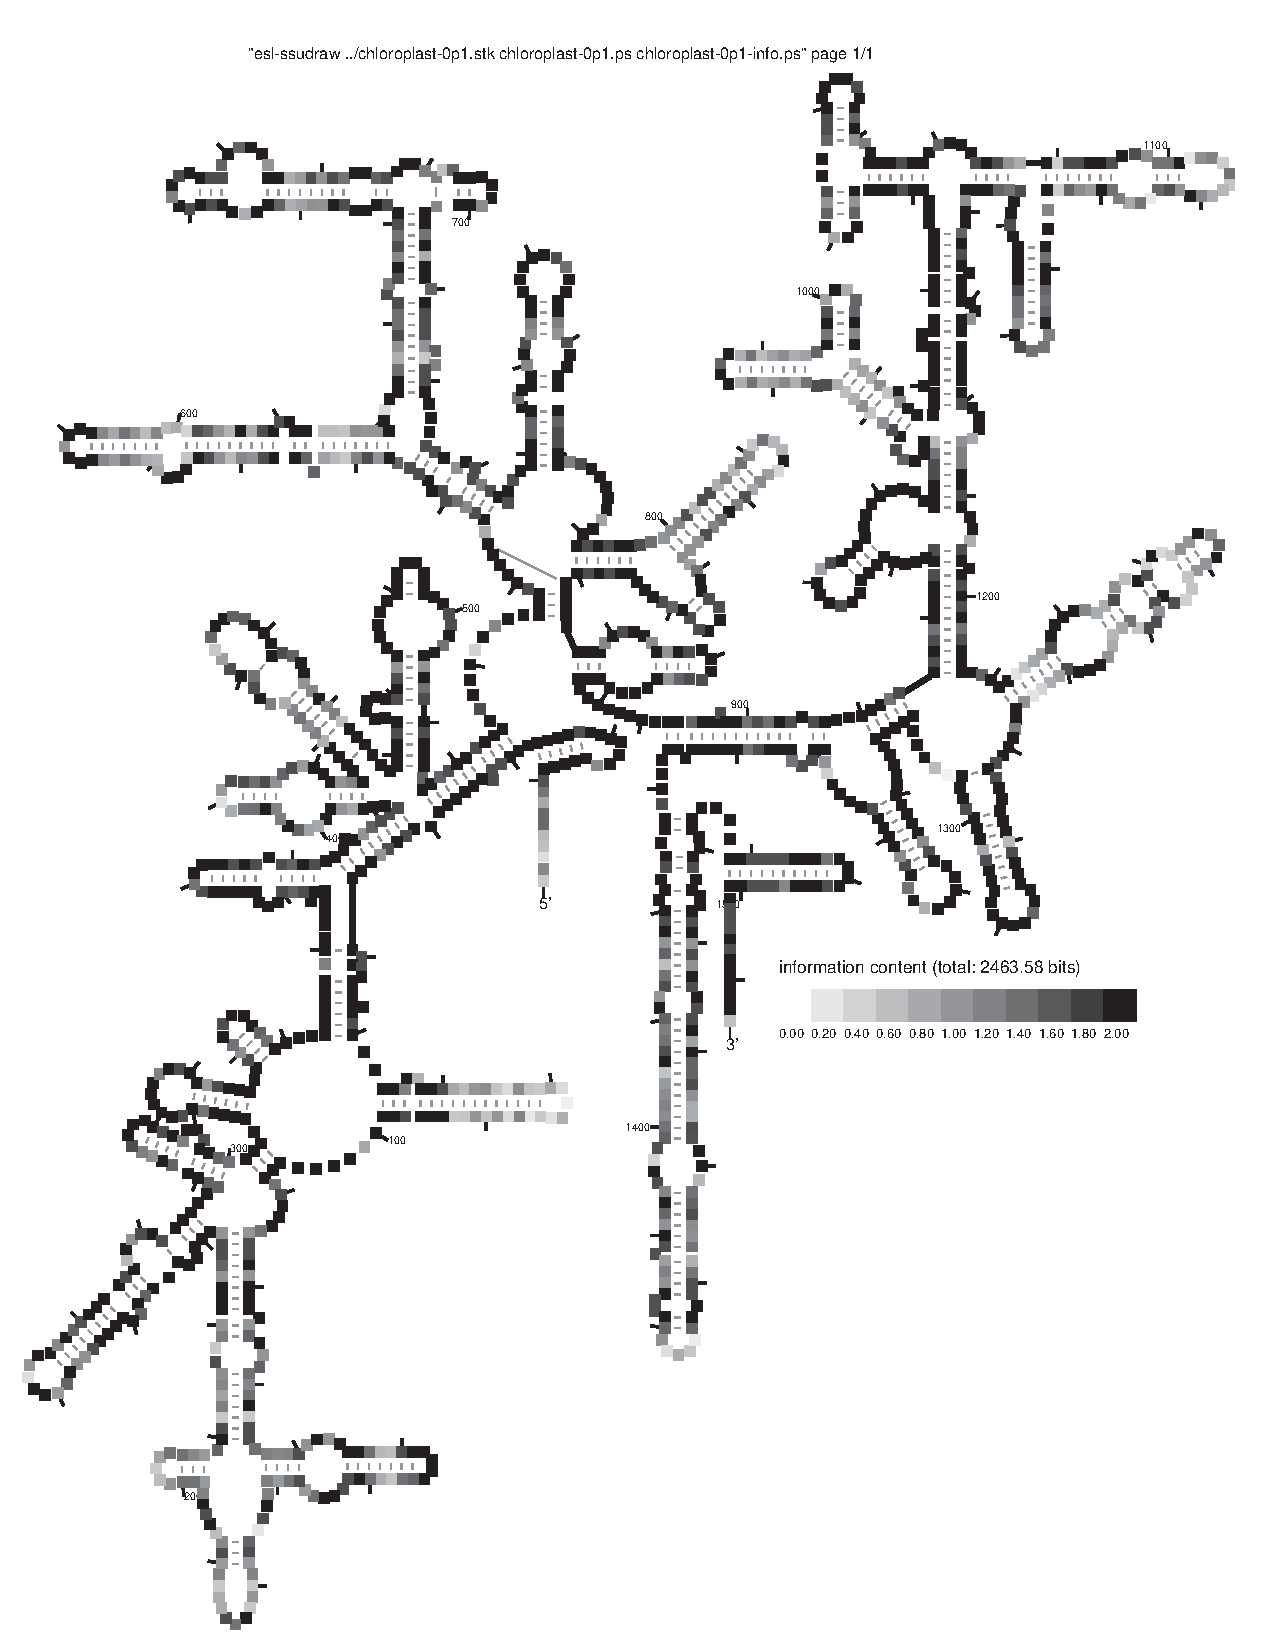
\includegraphics[height=8.5in]{../../seeds/ss-diagrams/chloroplast-0p1-info}
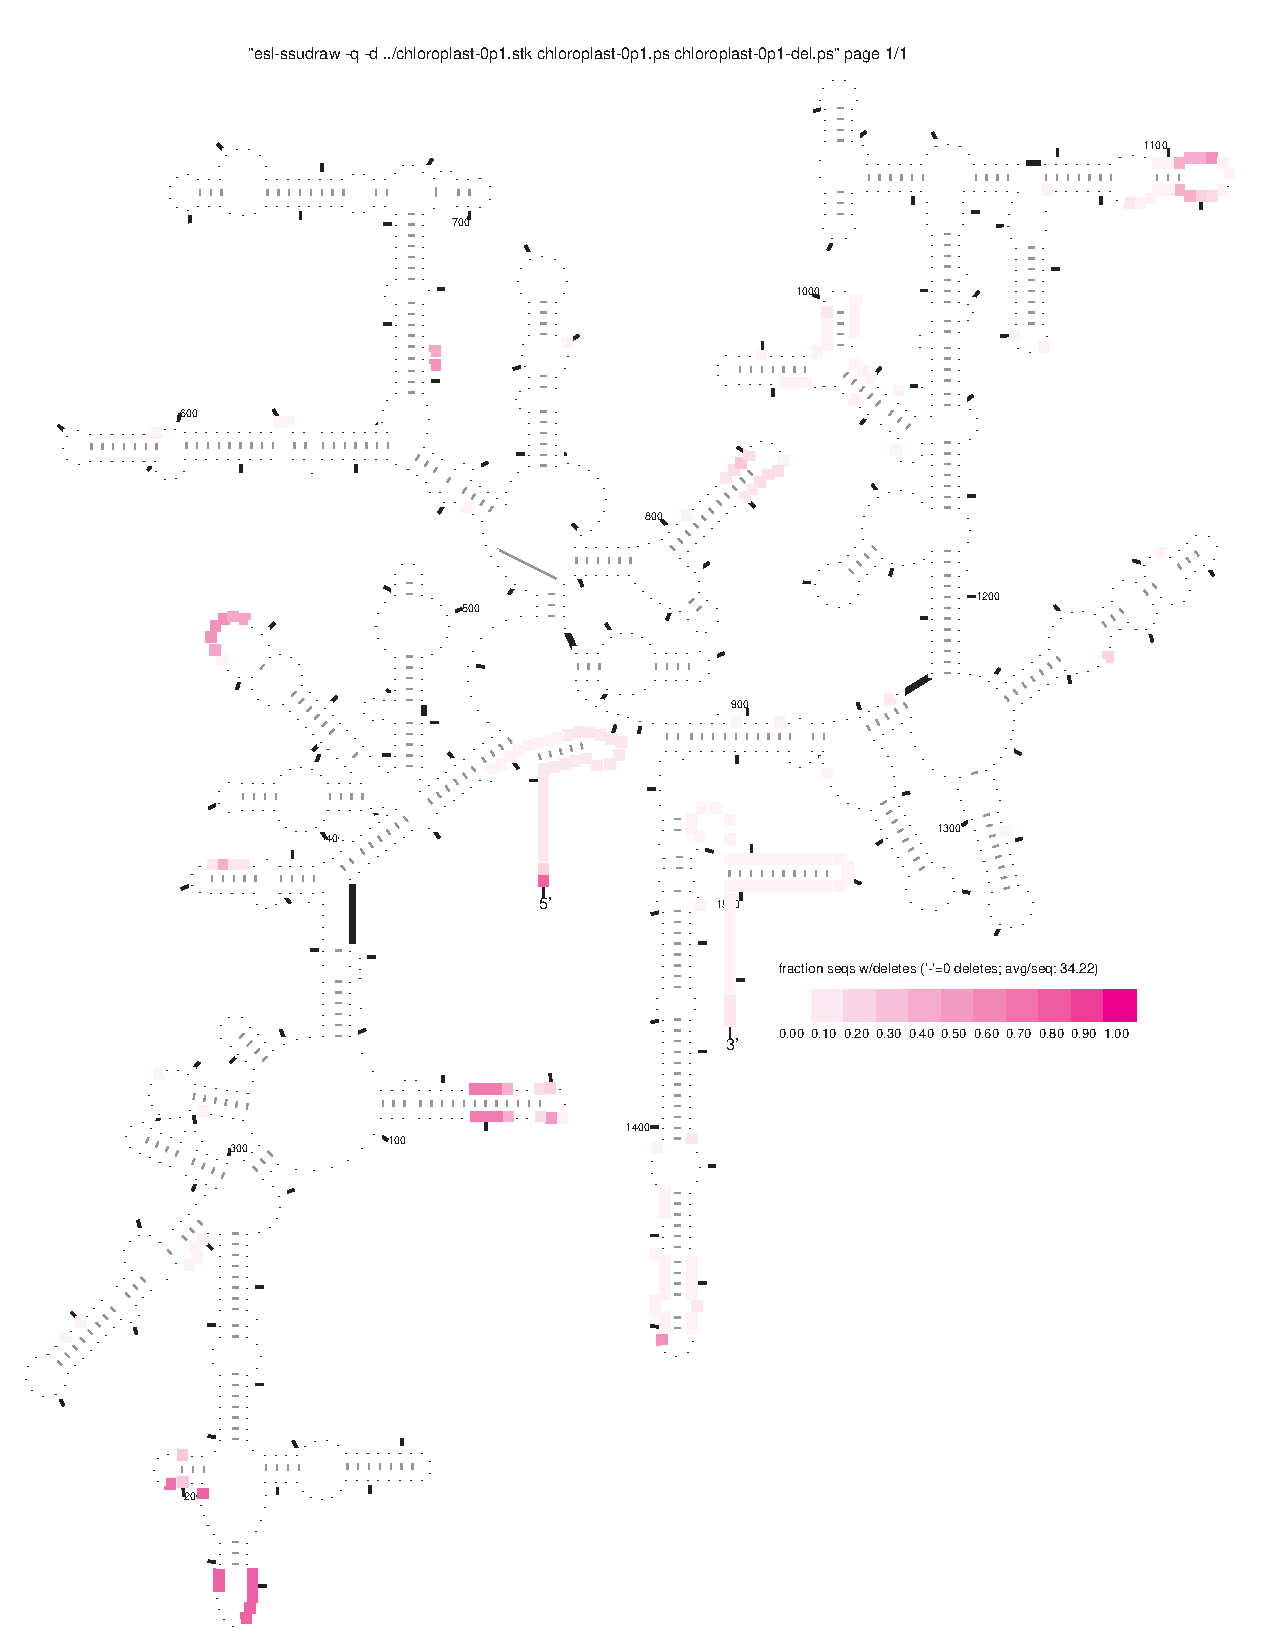
\includegraphics[height=8.5in]{../../seeds/ss-diagrams/chloroplast-0p1-del}
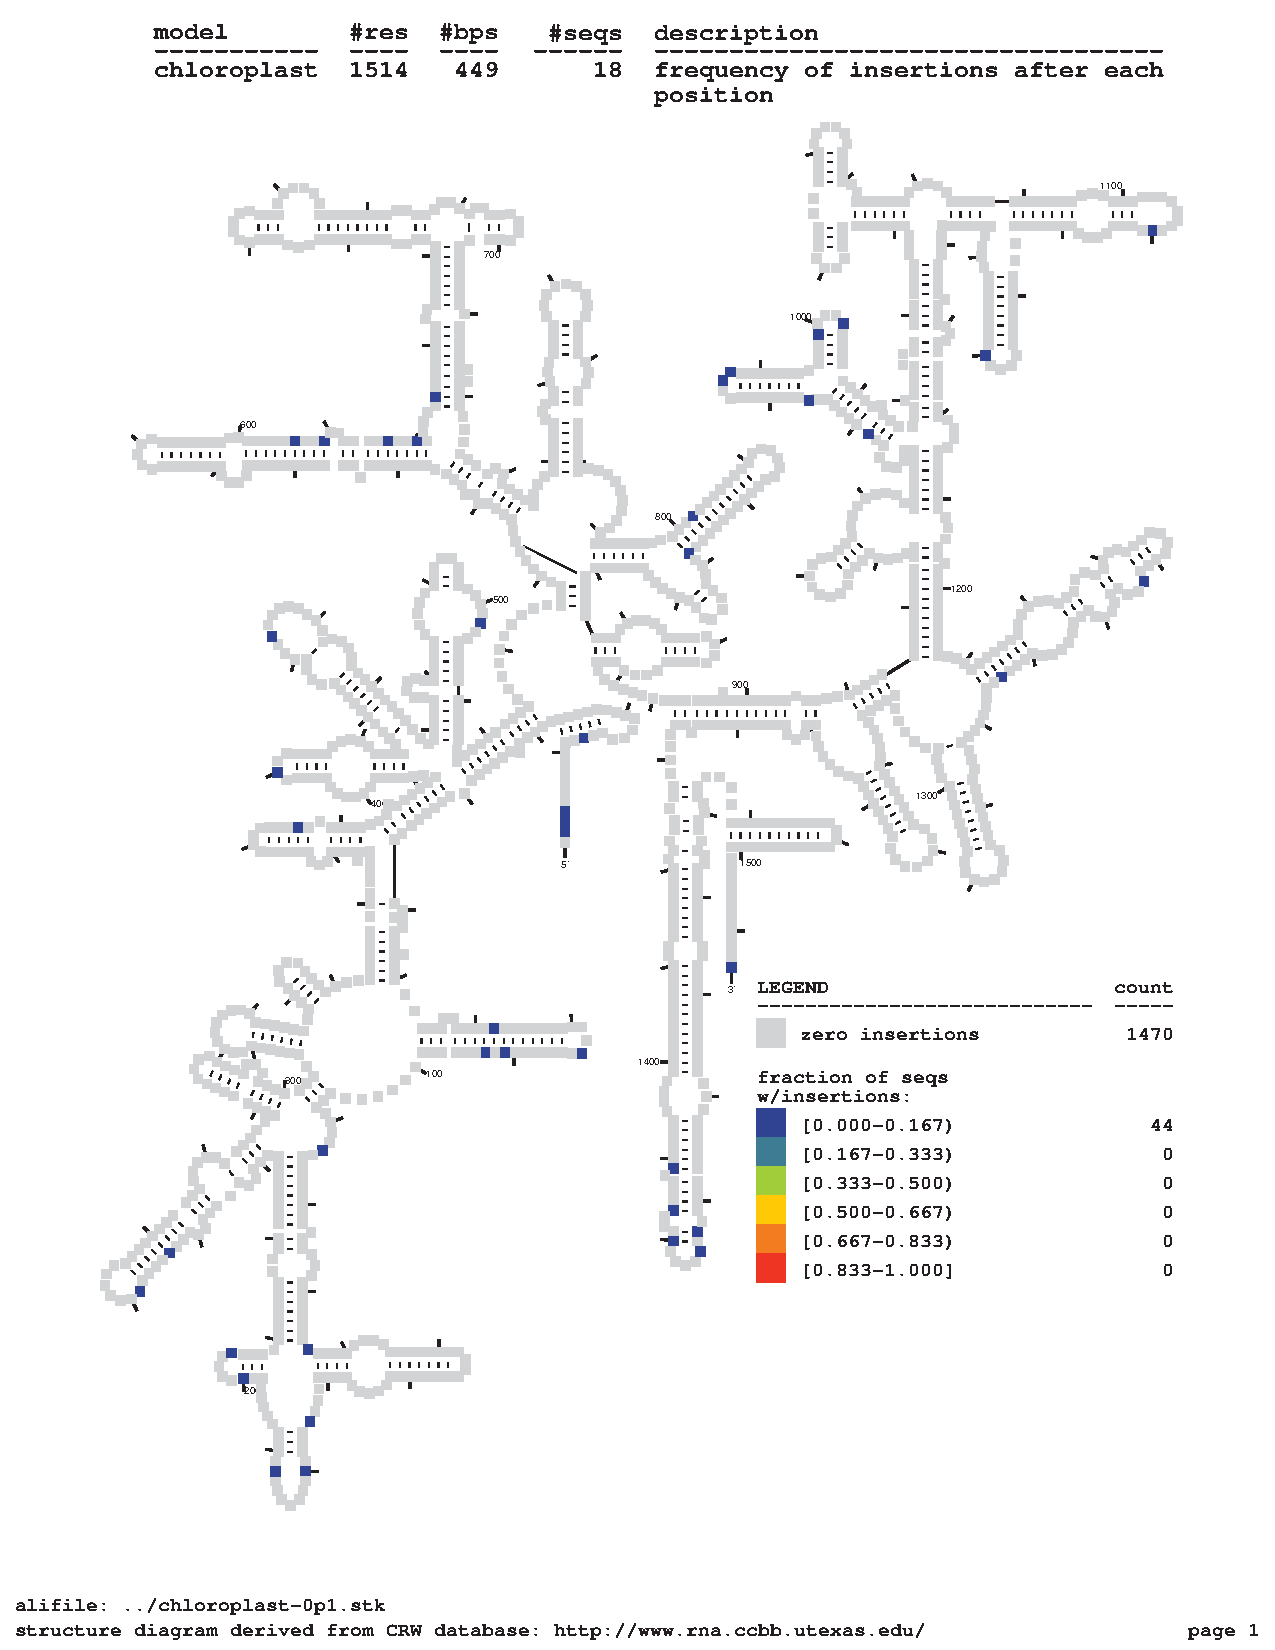
\includegraphics[height=8.5in]{../../seeds/ss-diagrams/chloroplast-0p1-ins}

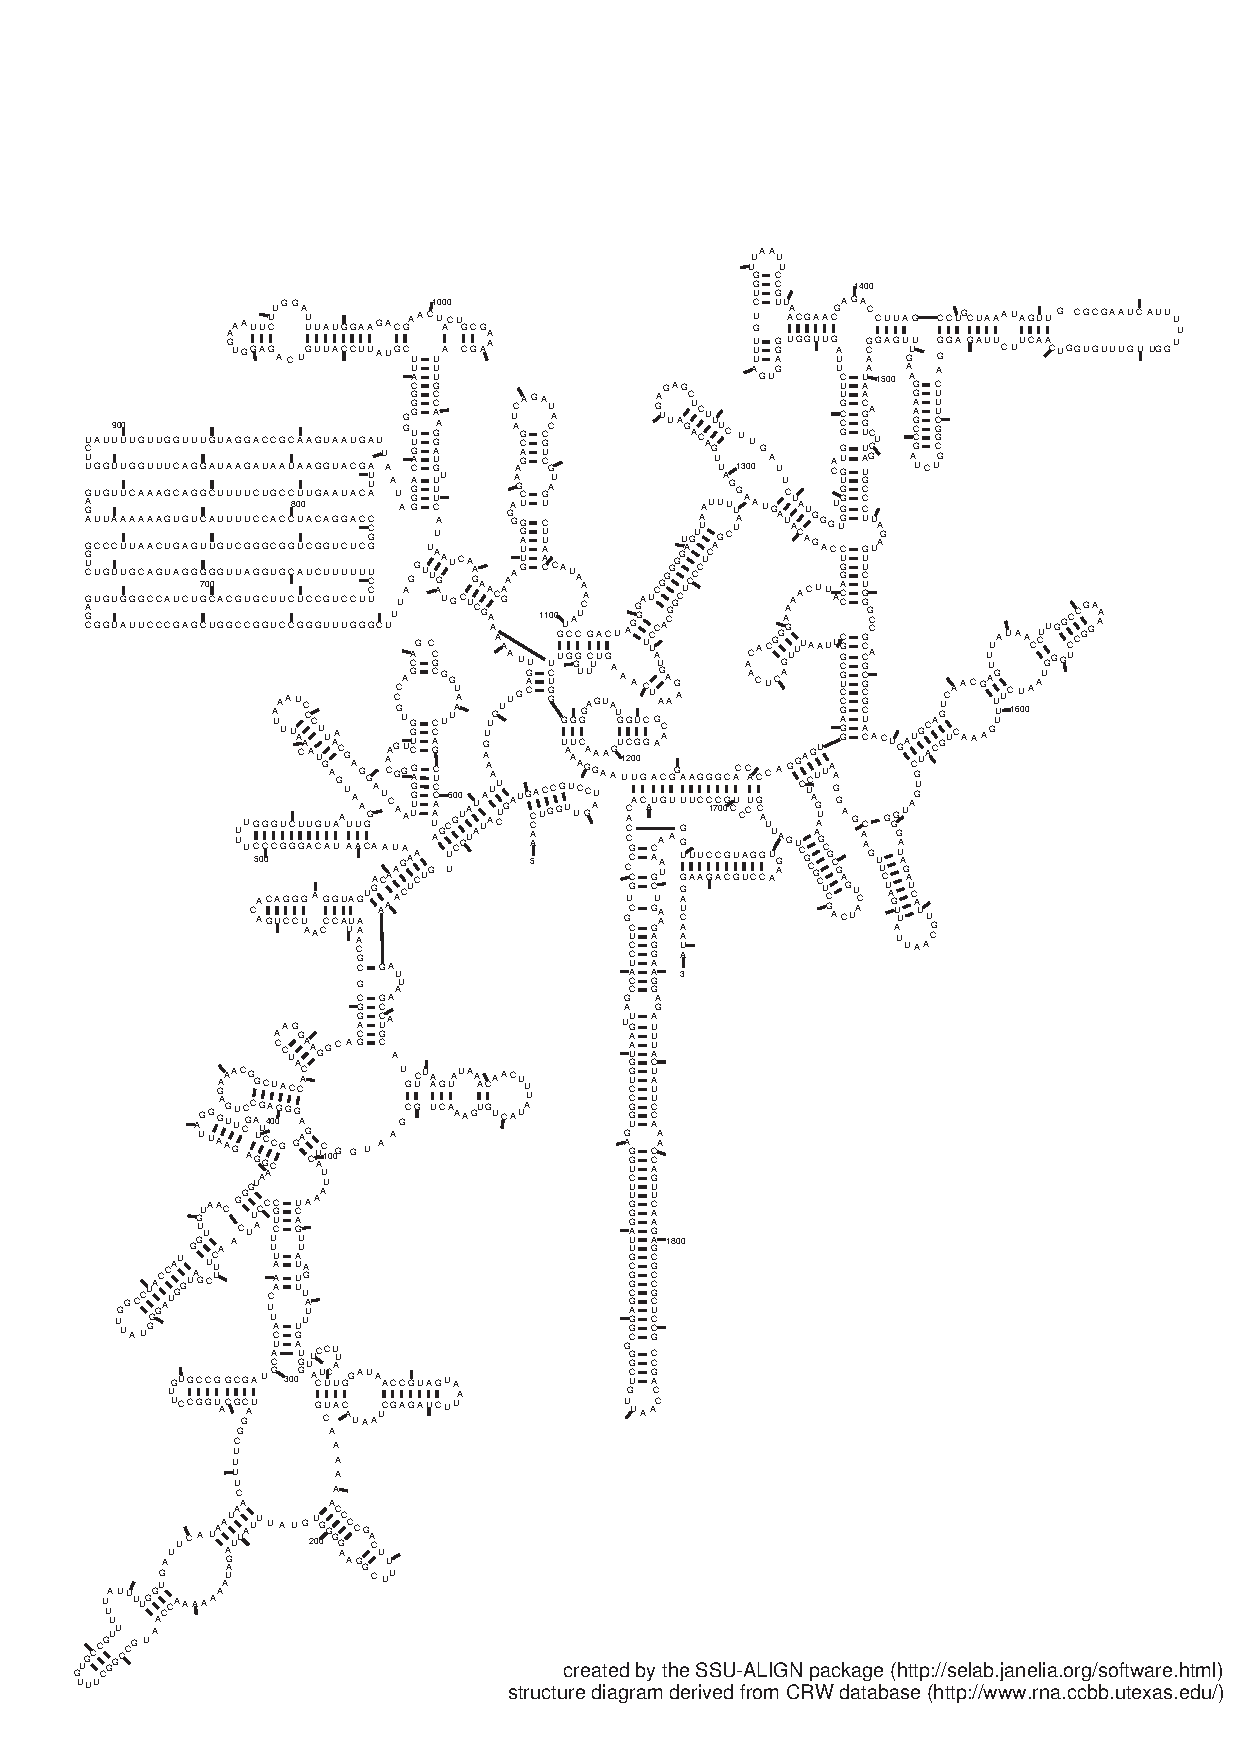
\includegraphics[height=8.5in]{../../seeds/ss-diagrams/eukarya-0p1}
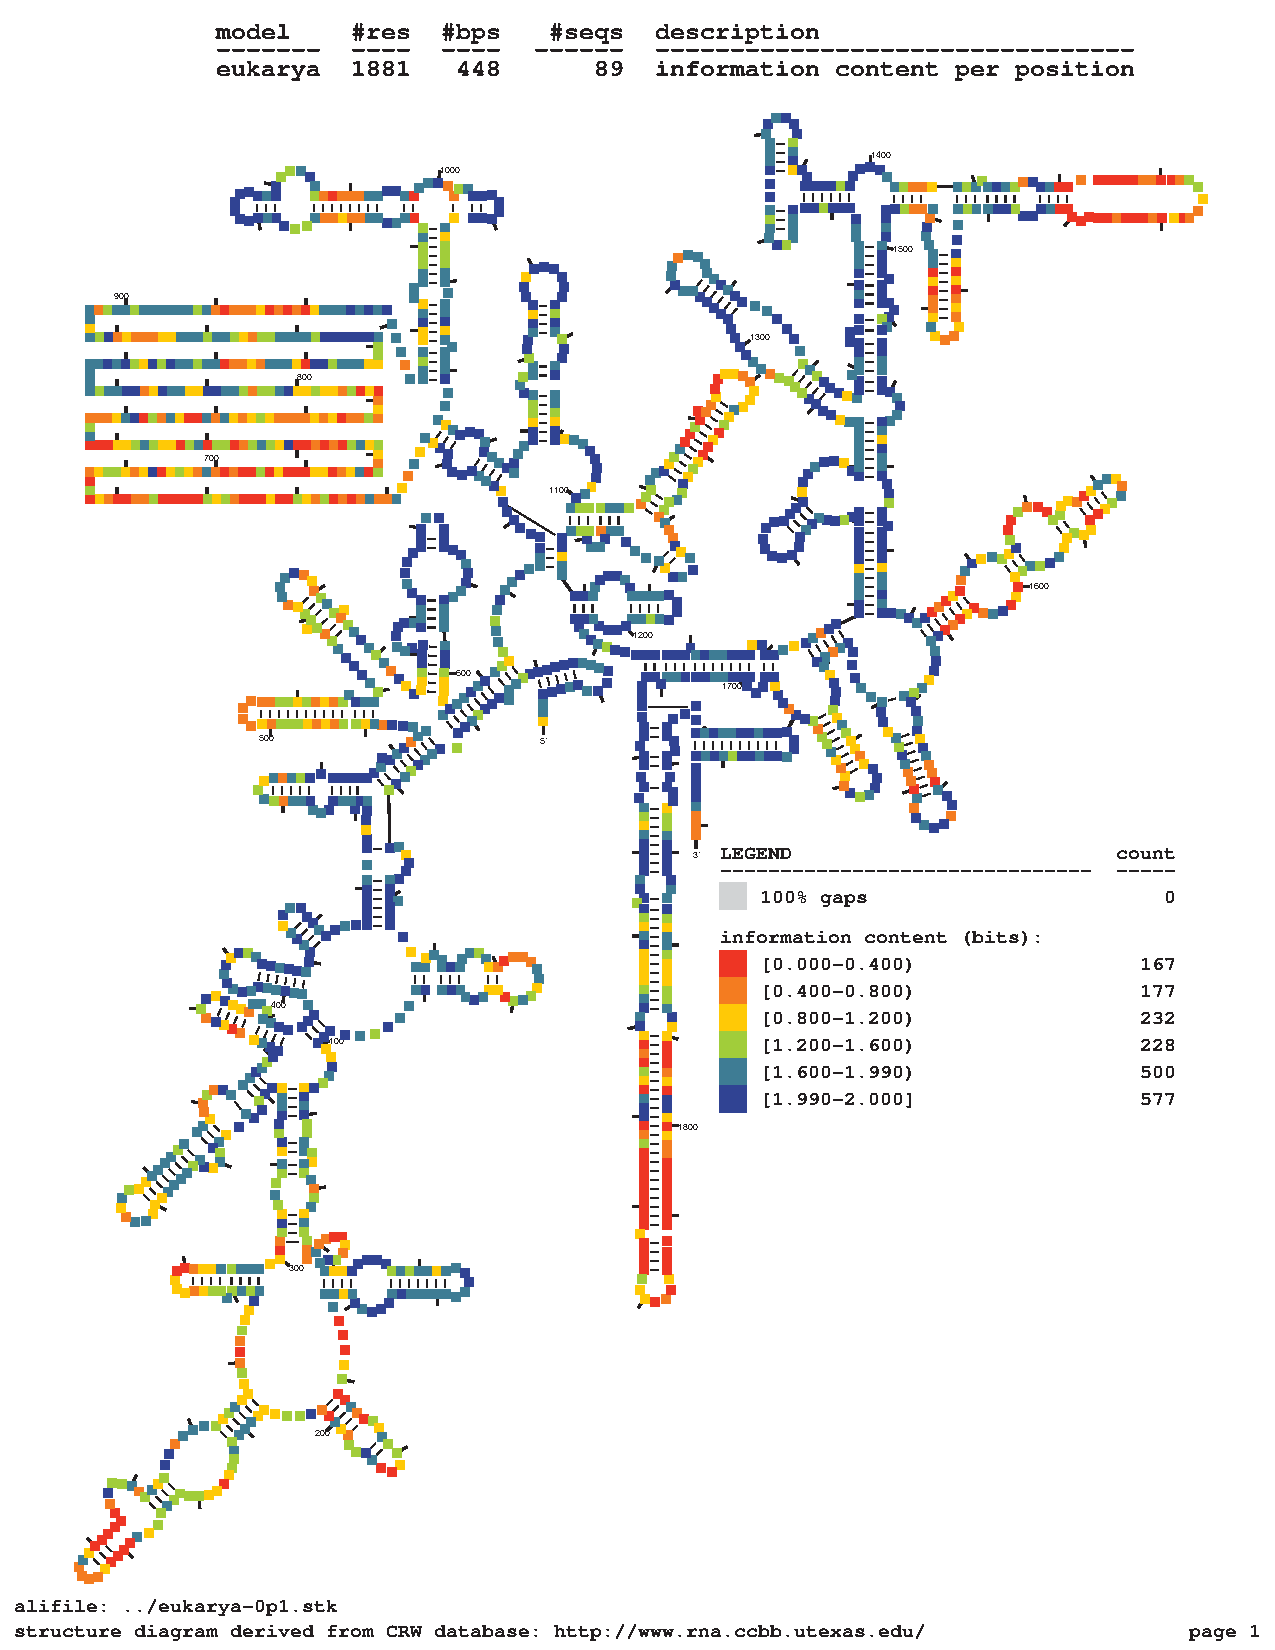
\includegraphics[height=8.5in]{../../seeds/ss-diagrams/eukarya-0p1-info}
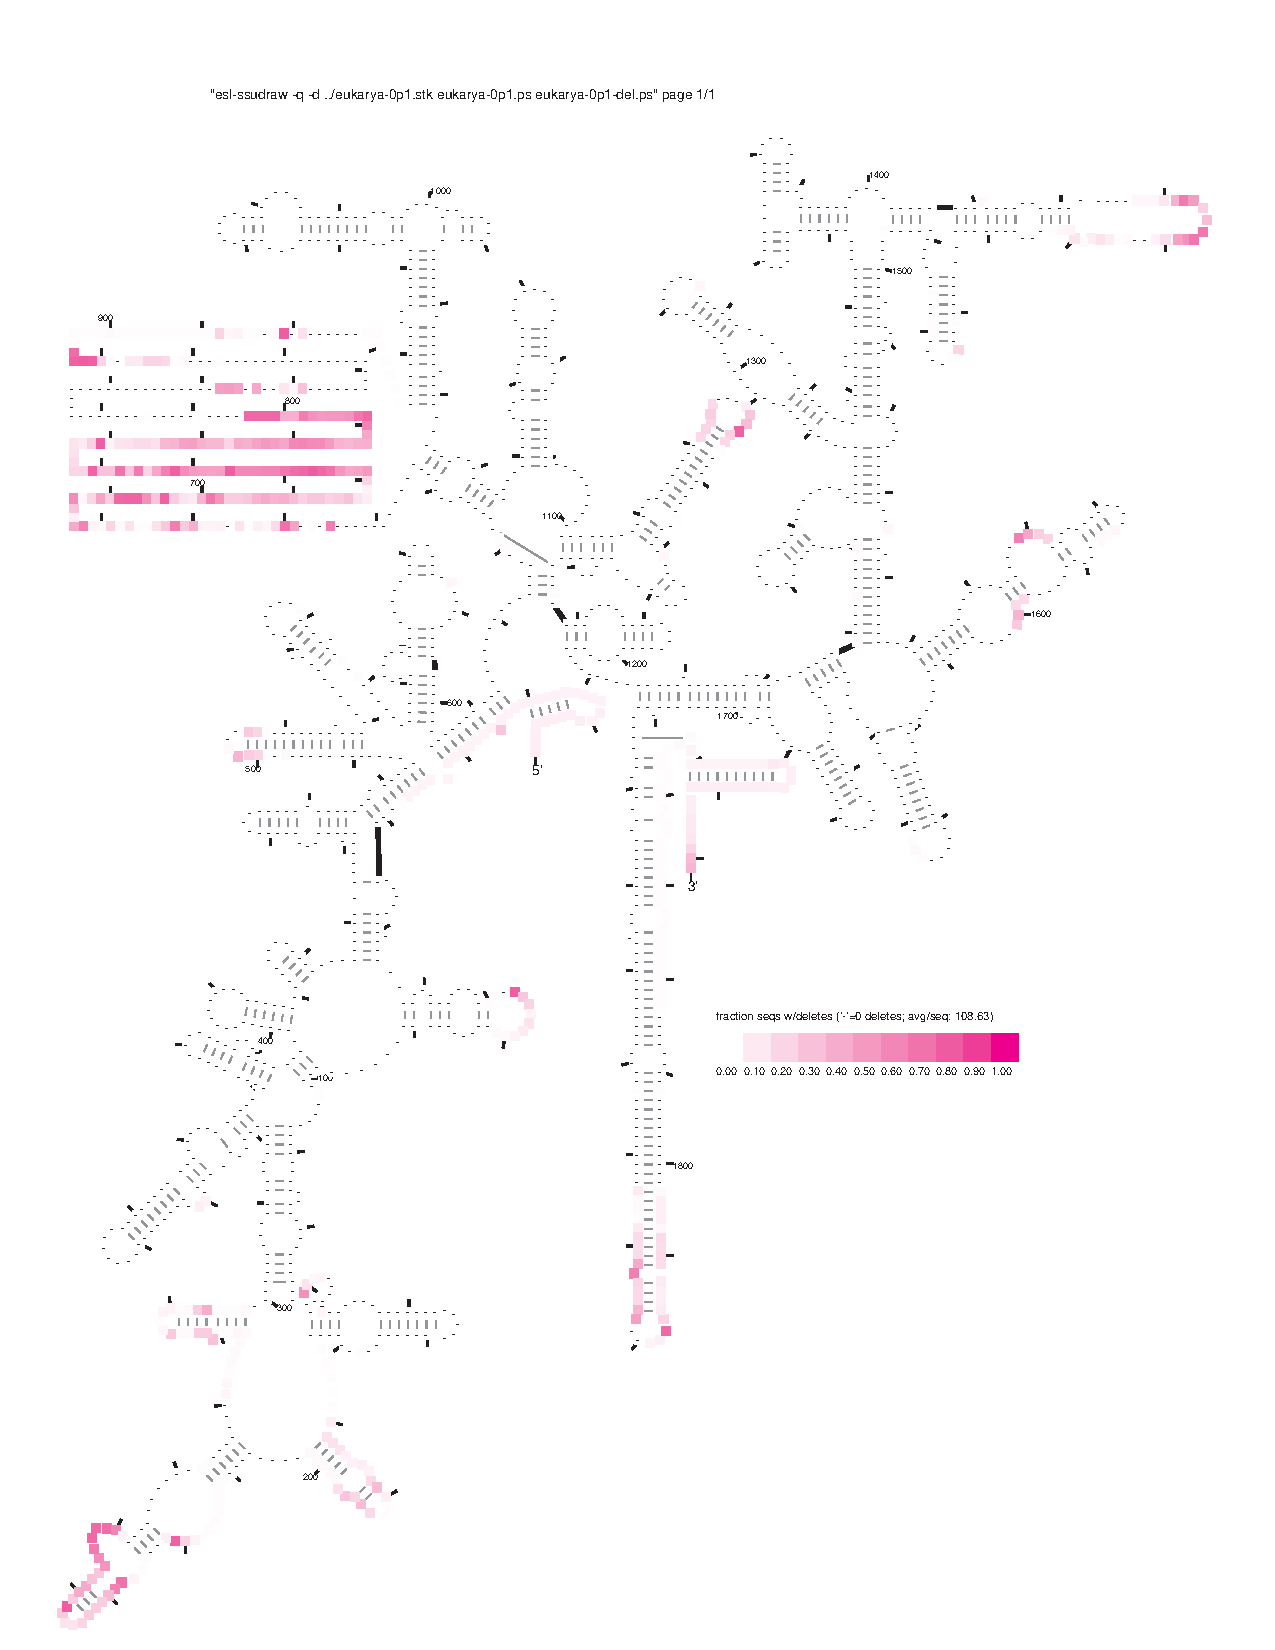
\includegraphics[height=8.5in]{../../seeds/ss-diagrams/eukarya-0p1-del}
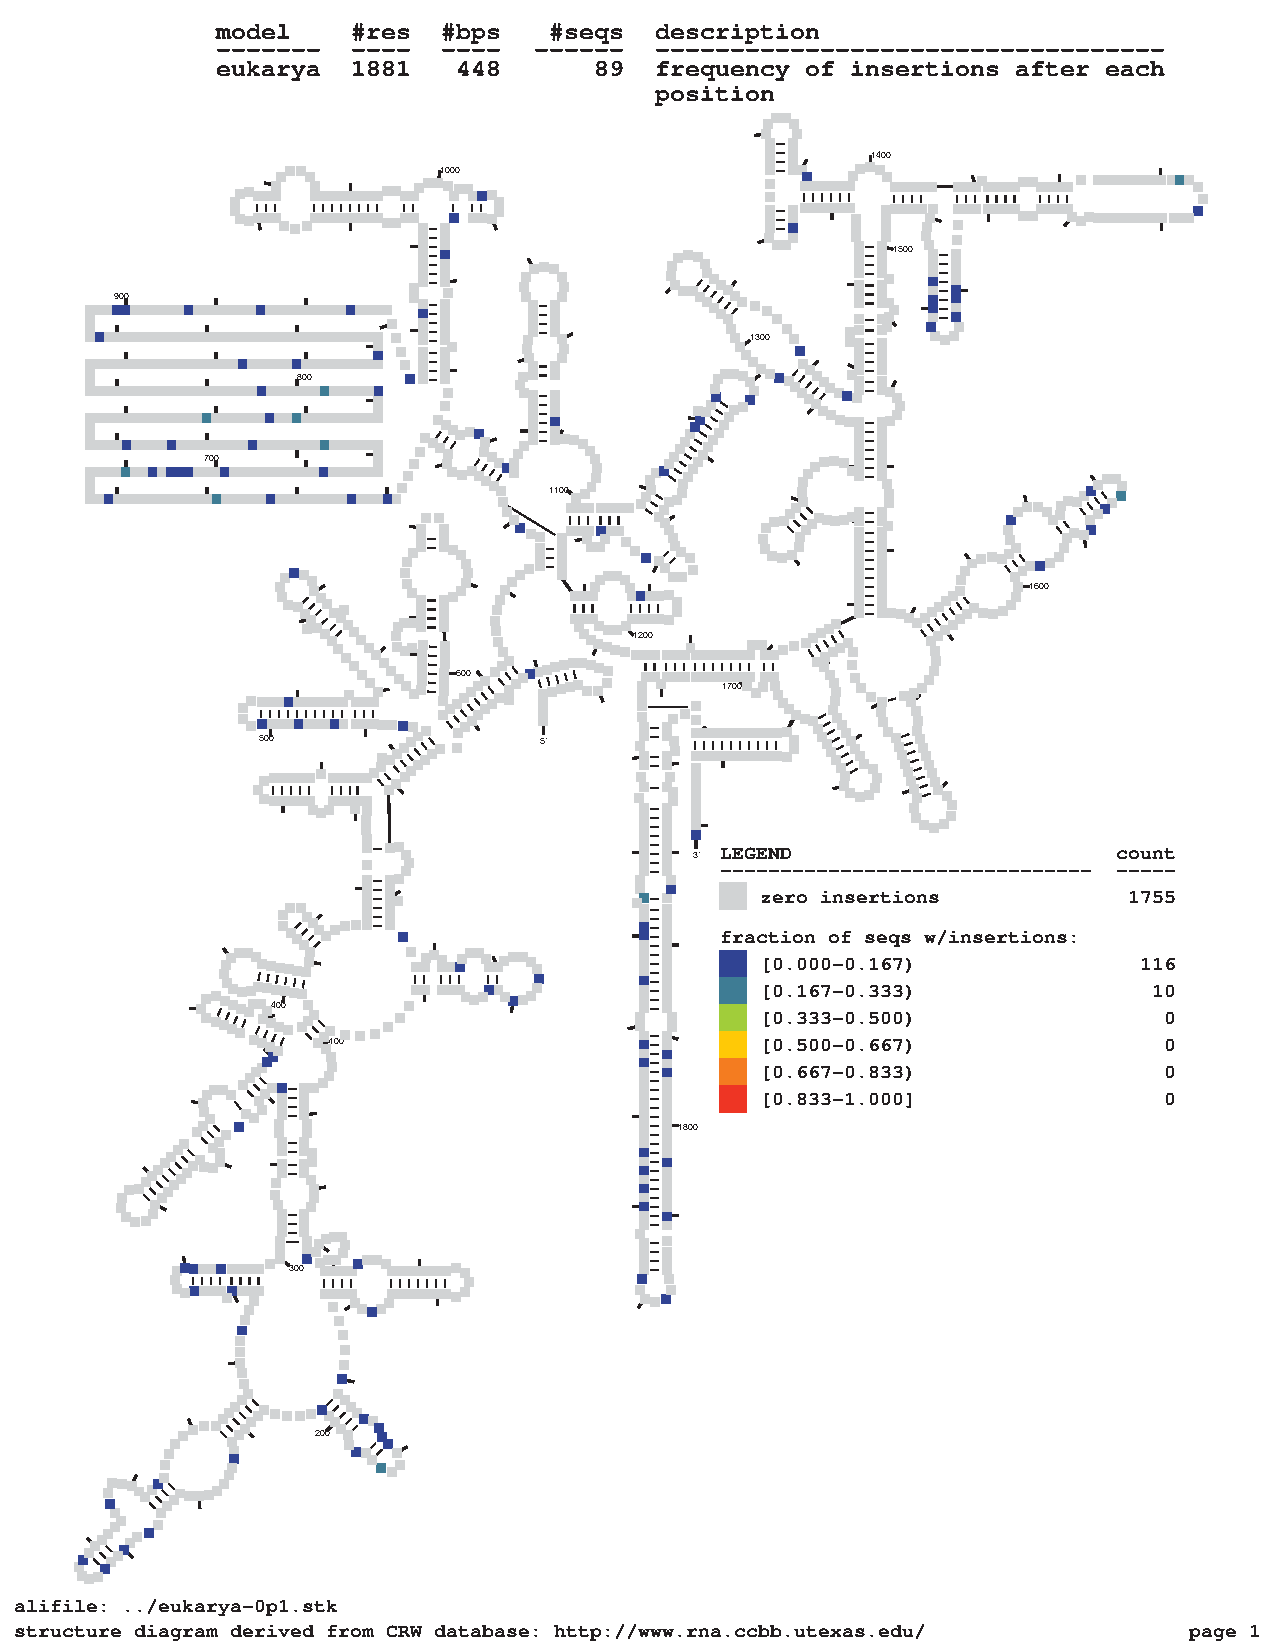
\includegraphics[height=8.5in]{../../seeds/ss-diagrams/eukarya-0p1-ins}

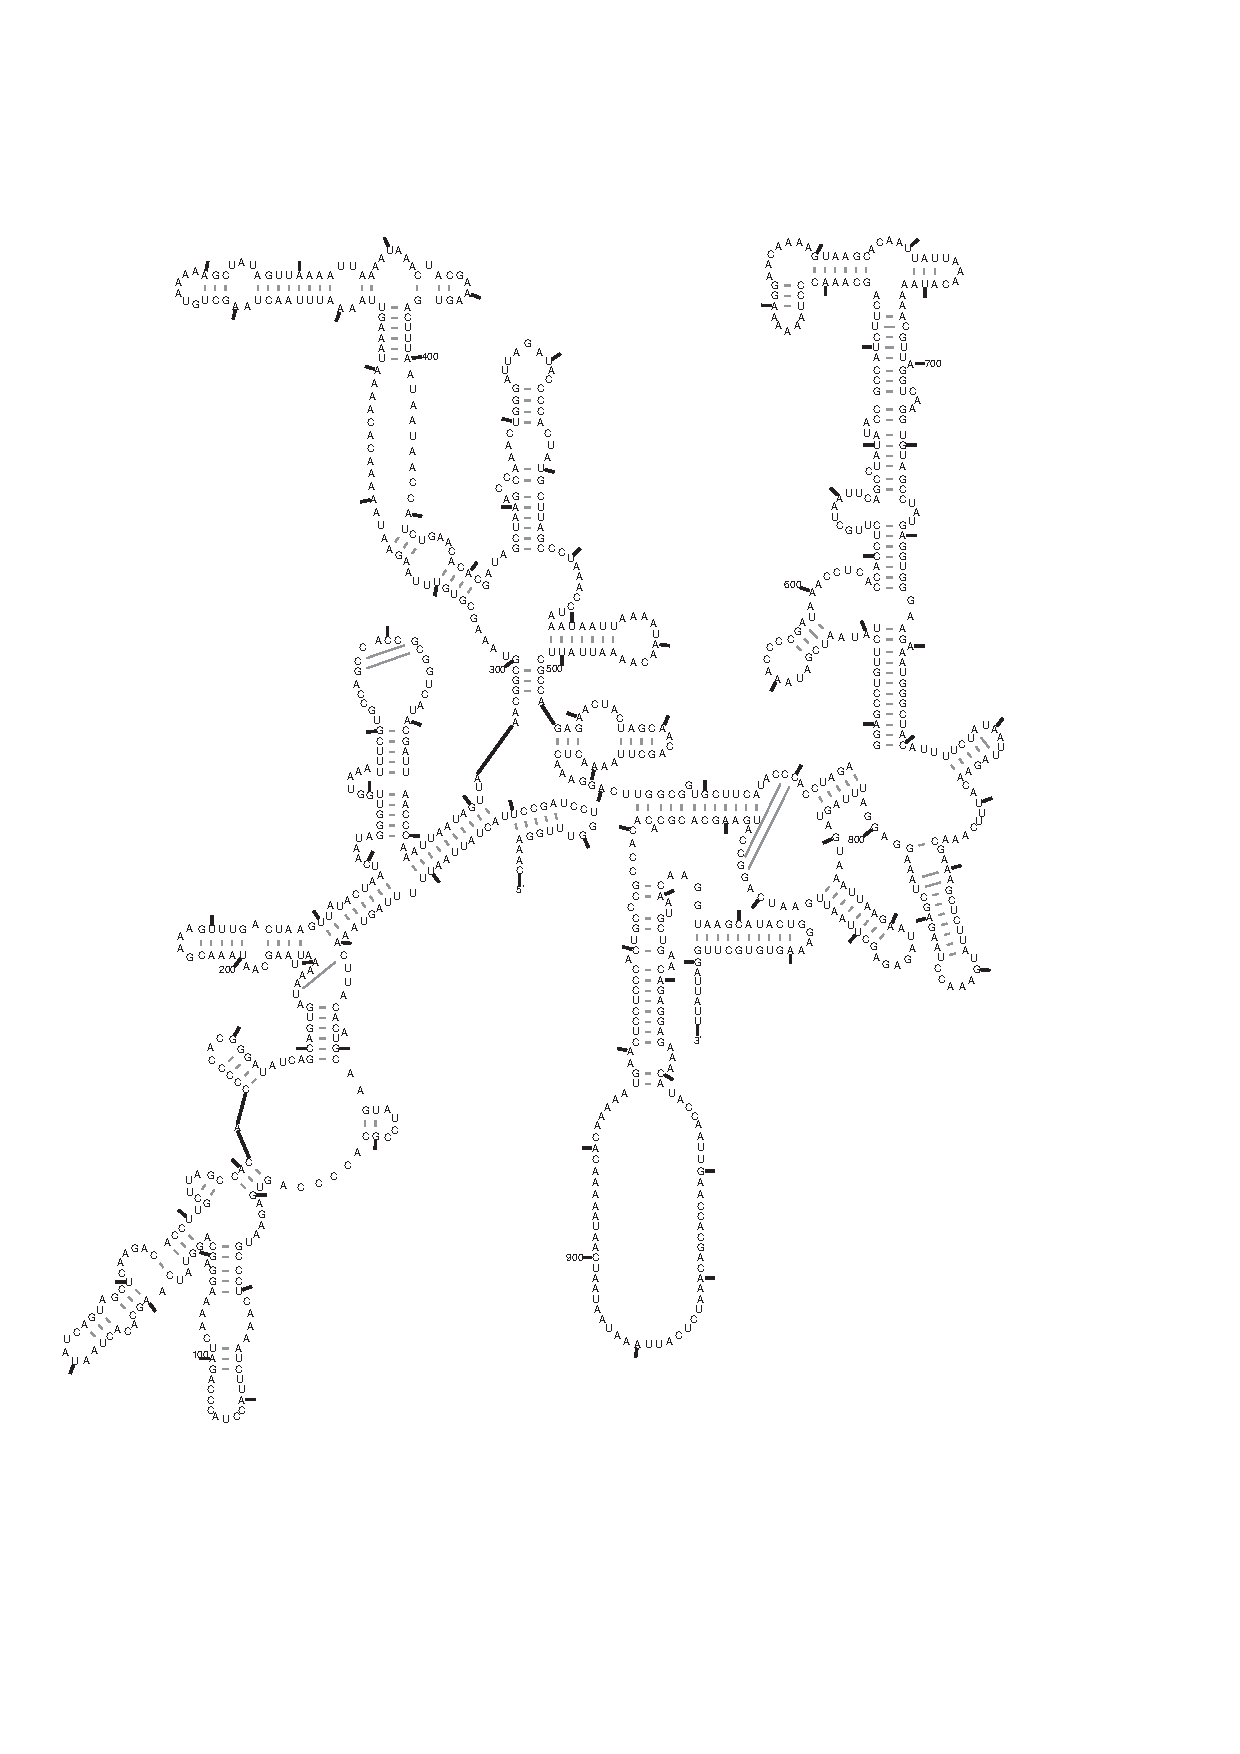
\includegraphics[height=8.5in]{../../seeds/ss-diagrams/metamito-0p1}
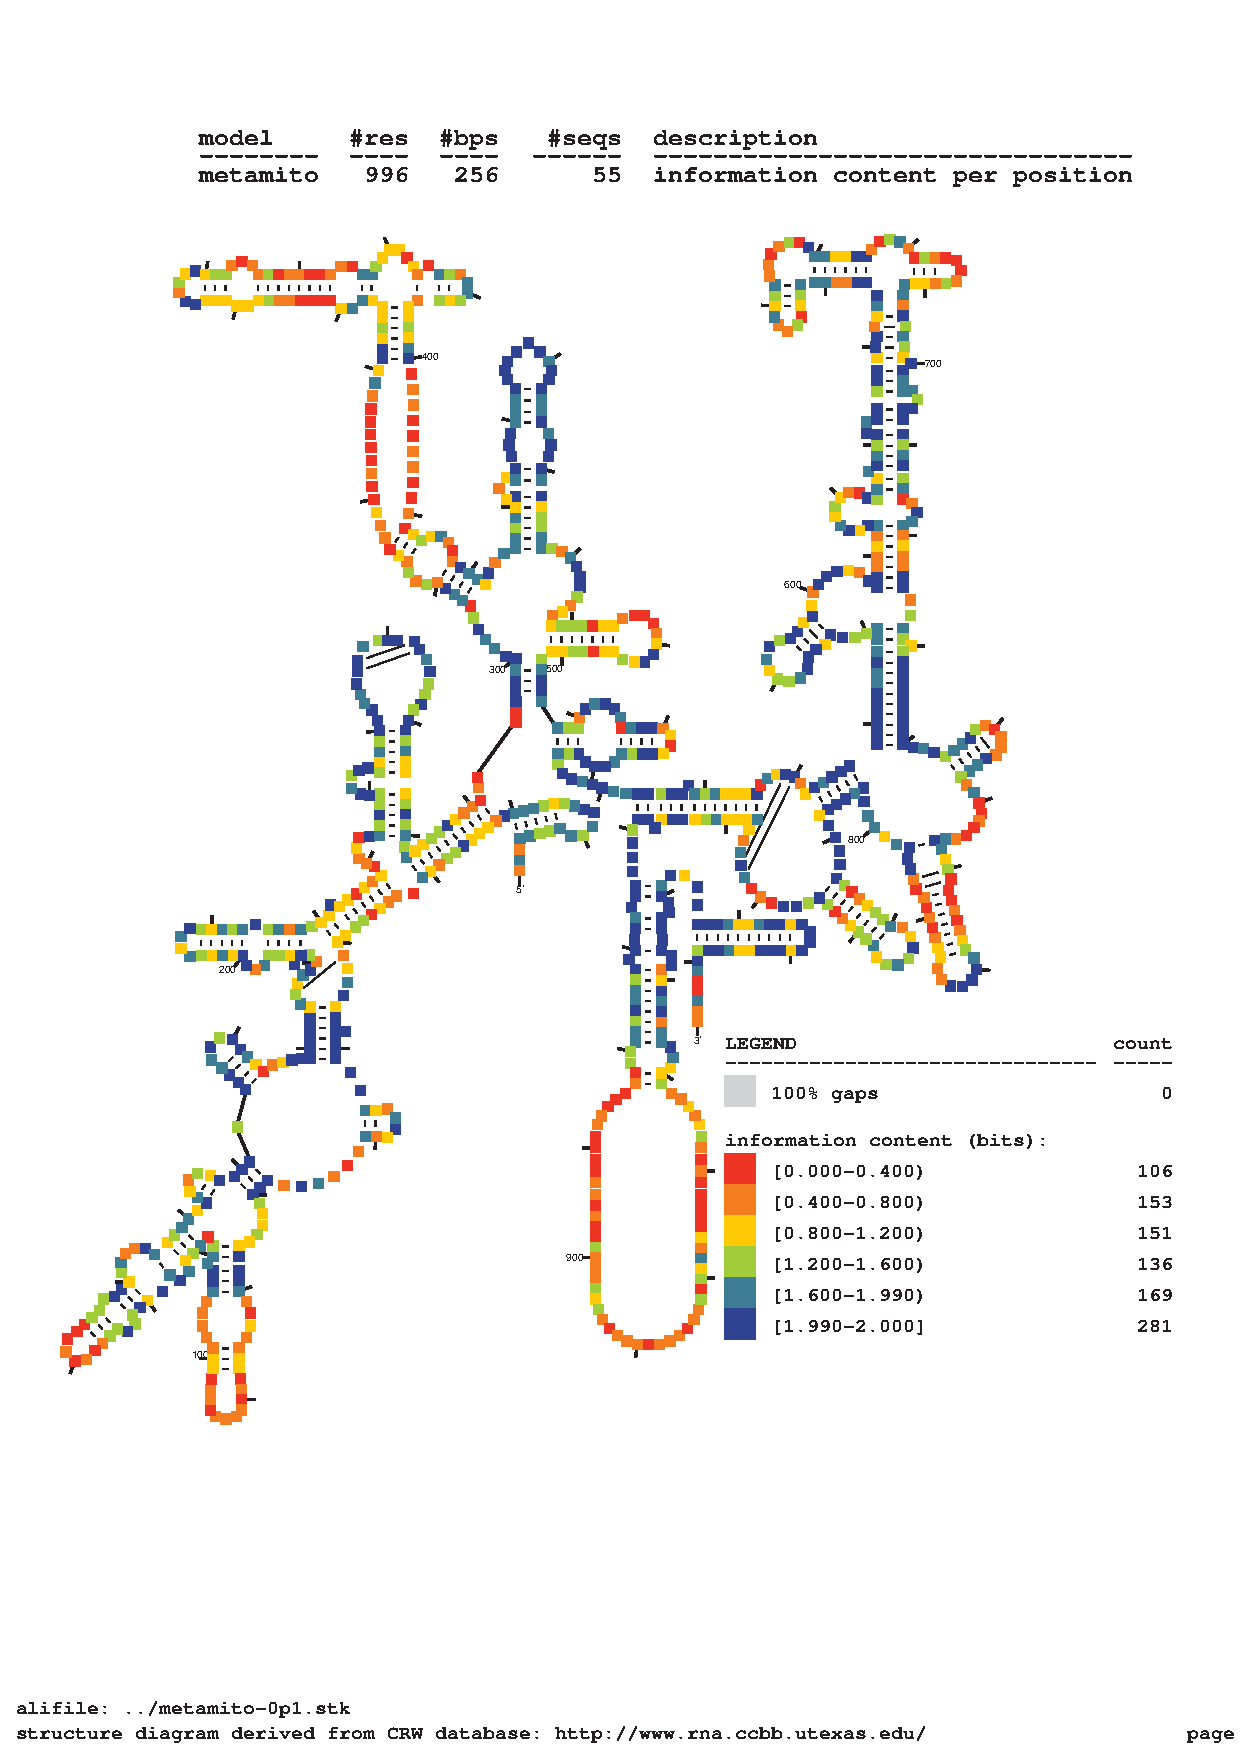
\includegraphics[height=8.5in]{../../seeds/ss-diagrams/metamito-0p1-info}
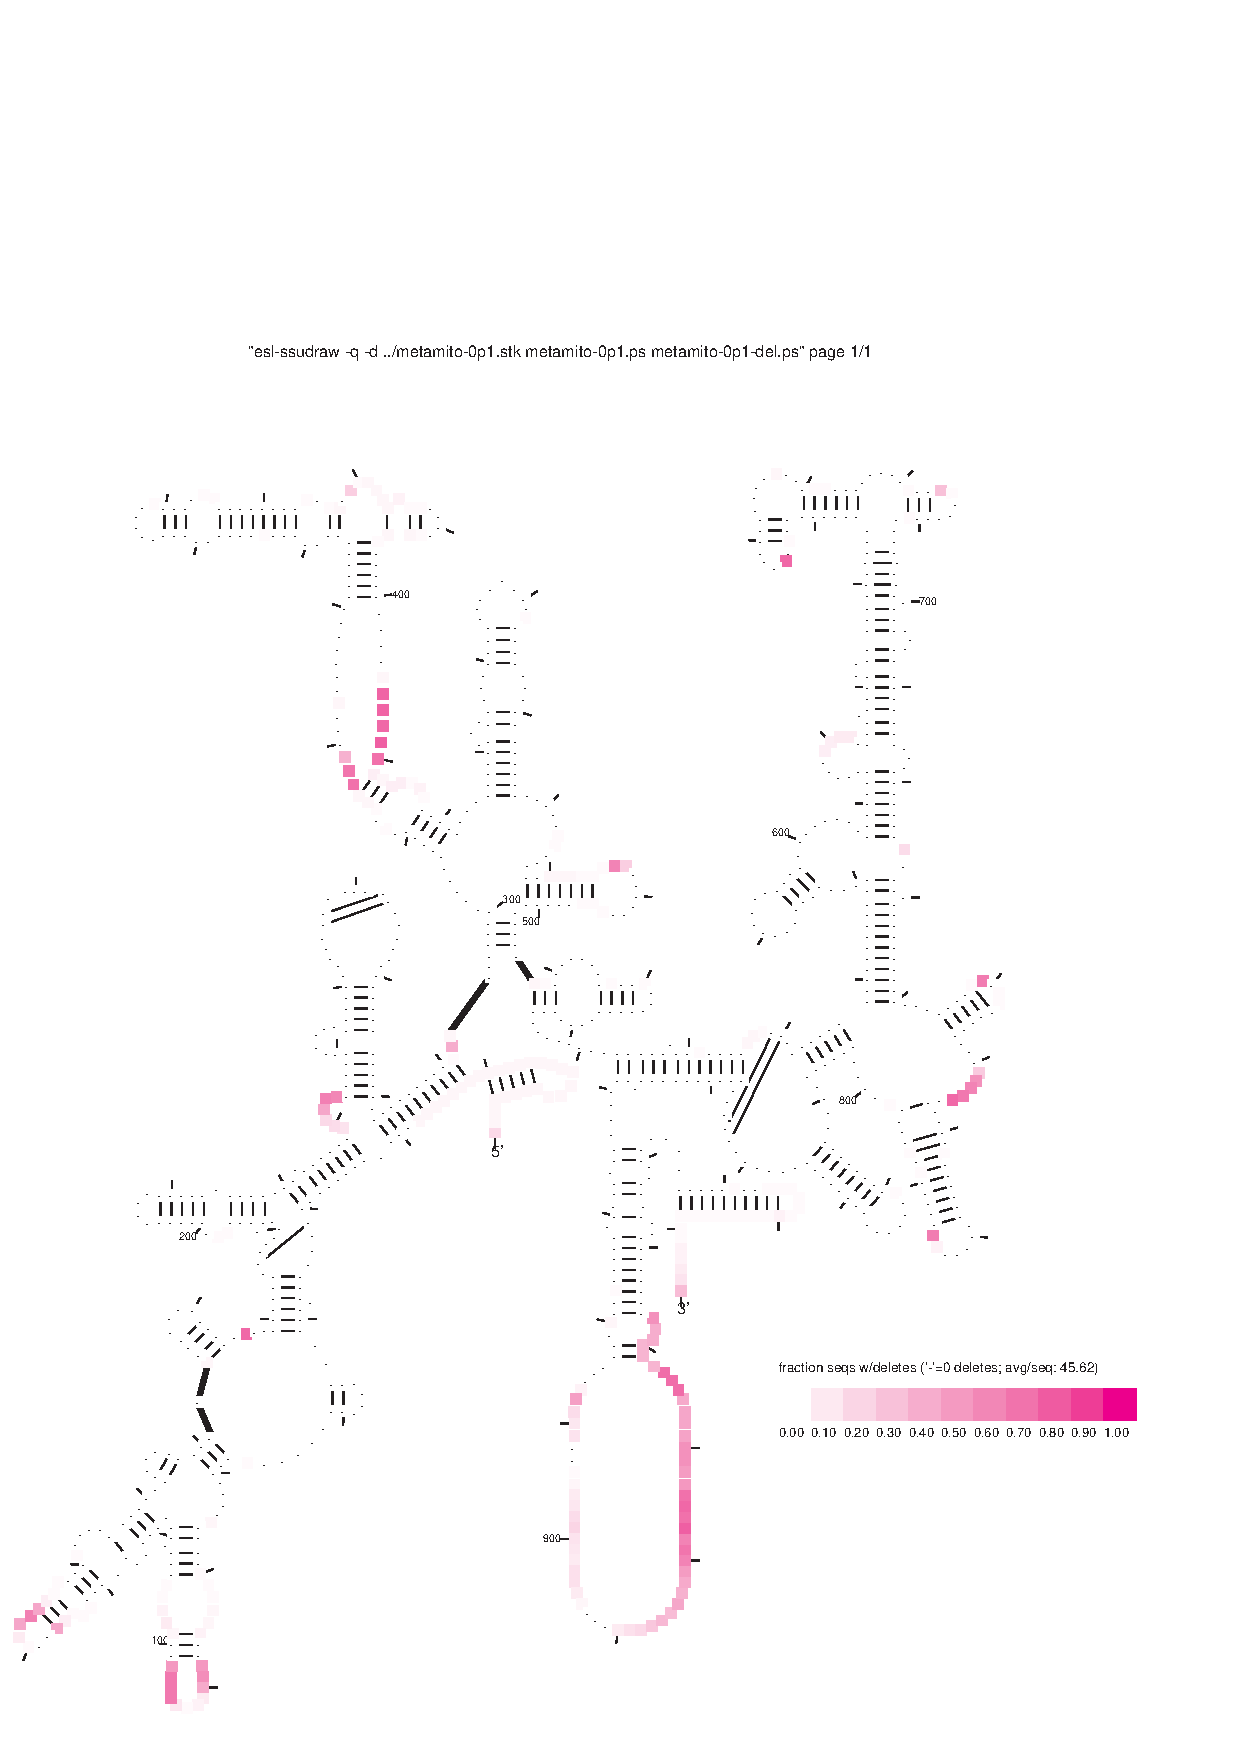
\includegraphics[height=8.5in]{../../seeds/ss-diagrams/metamito-0p1-del}
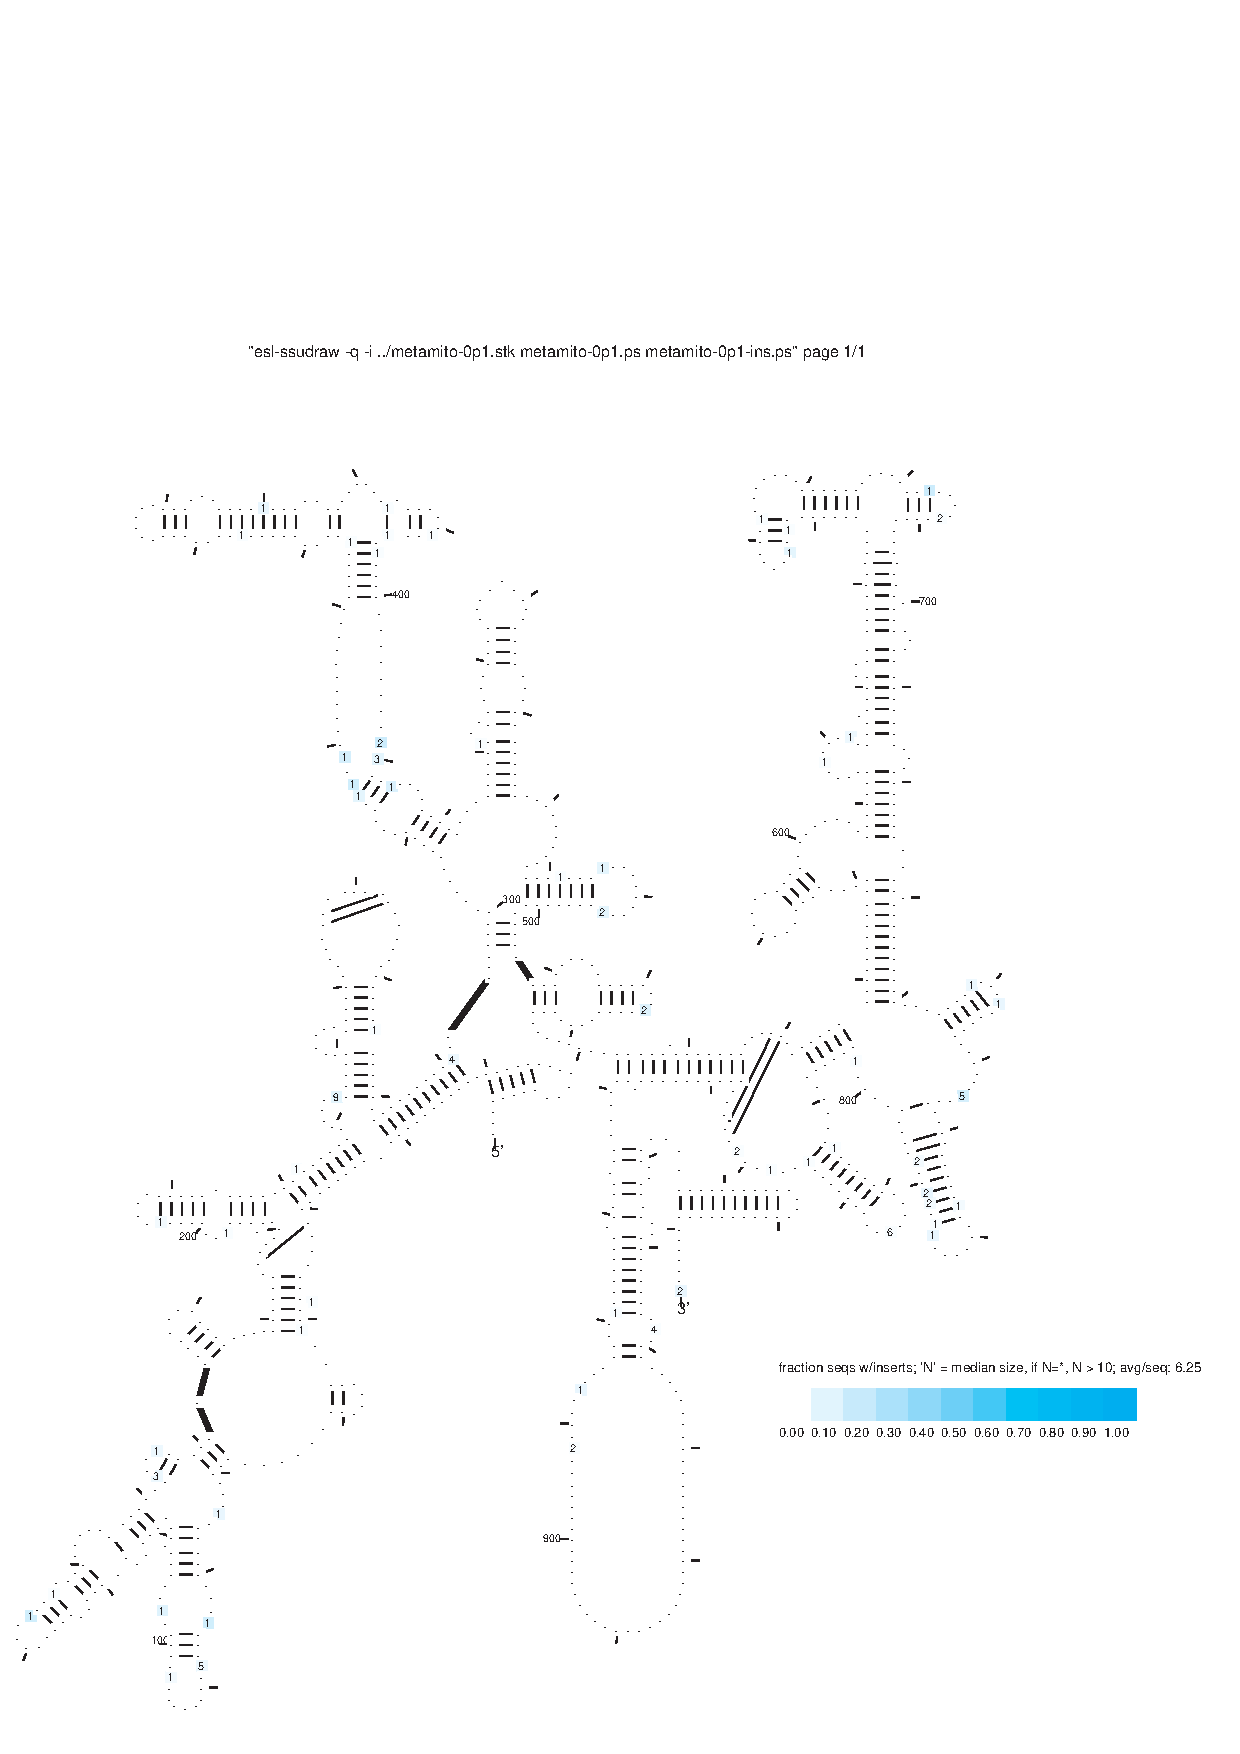
\includegraphics[height=8.5in]{../../seeds/ss-diagrams/metamito-0p1-ins}
\end{comment}

\subsection{Sequence diversity in the seed alignments}

TO DO: LIST HOW MANY SEQUENCES IN EACH PHYLA (or some other classification level)








